\documentclass[11pt,a4paper,twoside]{report}
\usepackage[left=2.00cm, right=2.00cm, top=1.00cm, bottom=2.00cm]{geometry}

%\usepackage[a4paper,headsep=10pt,top=3cm,bottom=3cm,inner=3.2cm,outer=2.2cm]{geometry}

\usepackage{microtype}
\usepackage[utf8]{inputenc}
\usepackage[T1]{fontenc}
\usepackage[bookmarks=false,colorlinks]{hyperref}
\usepackage{float}
\usepackage{listings}
\usepackage[official]{eurosym}
\usepackage{setspace}
\usepackage[table]{xcolor}
\usepackage{color}
\usepackage{rotating}
\usepackage{graphicx}
\graphicspath{{./images/}}
\usepackage[left=1.00cm, right=1.00cm, top=1.00cm, bottom=2.00cm]{geometry}
\author{Stéphane FEUGA\\{\small \href{mailto:sfeuga@member.fsf.org}{sfeuga@member.fsf.org}}}
\title{{\Huge Dossier de synthèse de pratique professionnel\\
Titre Développeur Logiciel}\\
{\normalsize Stage du 02/04/2014 au 31/05/2014 pour l'association Uncanny}}
\date {En date du 02/06/2014}

\hypersetup{pdftitle={DSPP, Titre DL}, pdfauthor={Stéphane FEUGA}, pdfsubject={Rapport de stage pour le Titre DPL}, urlcolor=blue, linkcolor=black}

\definecolor{lightgray}{rgb}{0.9,0.9,0.9}
\definecolor{darkgray}{rgb}{0.2,0.2,0.2}

\lstset{numbers=left, stepnumber=1, frame=single, breaklines=true, backgroundcolor=\color{lightgray}, tabsize=2, showstringspaces=false, captionpos=b, basicstyle=\scriptsize, literate=
			  {á}{{\'a}}1 {é}{{\'e}}1 {í}{{\'i}}1 {ó}{{\'o}}1 {ú}{{\'u}}1
			  {Á}{{\'A}}1 {É}{{\'E}}1 {Í}{{\'I}}1 {Ó}{{\'O}}1 {Ú}{{\'U}}1
			  {à}{{\`a}}1 {è}{{\`e}}1 {ì}{{\`i}}1 {ò}{{\`o}}1 {ù}{{\`u}}1
			  {À}{{\`A}}1 {È}{{\'E}}1 {Ì}{{\`I}}1 {Ò}{{\`O}}1 {Ù}{{\`U}}1
			  {ä}{{\"a}}1 {ë}{{\"e}}1 {ï}{{\"i}}1 {ö}{{\"o}}1 {ü}{{\"u}}1
			  {Ä}{{\"A}}1 {Ë}{{\"E}}1 {Ï}{{\"I}}1 {Ö}{{\"O}}1 {Ü}{{\"U}}1
			  {â}{{\^a}}1 {ê}{{\^e}}1 {î}{{\^i}}1 {ô}{{\^o}}1 {û}{{\^u}}1
			  {Â}{{\^A}}1 {Ê}{{\^E}}1 {Î}{{\^I}}1 {Ô}{{\^O}}1 {Û}{{\^U}}1
			  {œ}{{\oe}}1 {Œ}{{\OE}}1 {æ}{{\ae}}1 {Æ}{{\AE}}1 {ß}{{\ss}}1
			  {ç}{{\c c}}1 {Ç}{{\c C}}1 {ø}{{\o}}1 {å}{{\r a}}1 {Å}{{\r A}}1
			  {€}{{\EUR}}1 {£}{{\pounds}}1
			}

\begin{document}

\maketitle

\vspace*{\stretch{1}}
\begin{center}
This page intentionally left blank
\footnotetext{Ce document est rédigé en \LaTeX - l'intégralité de ce projet à été réalisé avec des outils sous licence libre}
\thispagestyle{empty}
\end{center}
\vspace*{\stretch{1}}

\tableofcontents

\chapter{Présentation}
	\section{Introduction}
		\paragraph*{}L'association Uncanny (loi 1901) est la forme juridique pour la Compagnie de danse du même nom. Cette structure a été créé lors de l'arrivé de Cédric Cherdel, Chorégraphe / Interprète sur Nantes. Outre la création et le développement des projets artistiques, cette association entend questionner la notion de « corporéité » dans la société, c'est-à-dire de ne plus penser la séparation du corps et de l'esprit, mais de percevoir cet engrenage incessant.\\
		Cette « corporéité », est questionné à travers le « uncanny\footnote{Uncanny ou Unheimlich (en Allemand) concept est ré-élaboré en 1919 par Freud. Ce dernier suppose (à partir de cas clinique d'obsessionnels ainsi que de la littérature) que l'origine de l'inquiétante étrangeté correspond au retour du même, du semblable. Par exemple, Freud voyageait dans un train, il se leva de sa banquette pour interpeller le contrôleur. Lorsqu'il se leva, il vit un homme, à l'extérieur de son compartiment, à la silhouette antipathique, désagréable, voire inquiétante. Cet homme qu'il apercevait sans réellement distinguer ses traits était en fait son reflet que lui renvoyait la vitre de la porte. Dans cet exemple, on voit bien le retour du semblable, du reflet. Cette image d'abord dérangeante devient, une fois identifiée, la sienne.} », ce concept divise autant qu'il assemble.
		\paragraph*{}Après des études de cinéma à l'université de Montpellier, Cédric Cherdel intègre le master professionnel d'arts de la représentation à Tours. C'est dans ce cadre qu'il rencontre Véronique Solé qui dirige et chorégraphie le groupe de recherche chorégraphique de Tours qui l'invite à intégrer ce groupe. Dans ce contexte tourangeau, Cédric va développer et ouvrir ses pratiques chorégraphiques notamment auprès du projet artistique Bernardo Montet (CCN de Tours) et des artistes invités a participé à celui-ci : Thomas Ferrand, Thierry Bae, Susan Buirges...\\
		En 2010, il intègre la licence professionnelle initiée par Maguy Marin « De l'interprète à l'auteur » au CCN de Rillieux la Pape puis en 2011, le master Essai, performance et chorégraphie au CNDC d'Angers, direction artistique Emmanuelle Huynh. En 2012, il s'installe à Nantes et Fonde l'association Uncanny.\\
		Il se forme à partir de 2010 au Reiki, soin énergétique japonais crée par le Dr Usui puis en 2012, au massage Nuad Bo Rarn (style du nord) à L'International Training Massage à Chang Mai, Thaïlande.
	\section{Compétences à mettre en œuvre}
		\paragraph*{\indent Compétence Obligatoire :} Développer une interface utilisateur (page 19 du REAC et page 8 du RC).
		\paragraph*{\indent Compétence Choisie :} Mettre en œuvre une solution de gestion de contenu ou d’e-commerce (page 22 du REAC et page 8 ru RC).
		\newpage
	\section{Remerciements}
		\paragraph*{}Tout d'abord, je souhaite  remercier M. Cédric CHERDEL et M. Laurent CEBE de l'association Uncanny qui m'ont offert la possibilité d'avoir un sujet de stage en adéquation avec mes capacités et les compétences à mettre en œuvre pour la validation de ce stage.
		\paragraph*{}Je souhaite aussi remercier Gabriel BLOCK, Emanuelle FERRAND, Erwan FOURNEL et Florence \linebreak NATIVELLE, de l'I.M.I.E., pour leurs implications et leurs aides tout au long de cette formation.
		\paragraph*{}Je souhaite enfin remercier Ada Lovelace\footnote{\url{https://fr.wikipedia.org/wiki/Ada\_Lovelace}} sans qui nous ne serions pas là.

\chapter{Mission}
	\section{Présentation du projet}
		Le projet est la mise en place de deux sites internet pour promouvoir les projets et activités de l'association Uncanny et plus particulièrement de Cédric Cherdel. 
		\subsection{Objectifs}
			\begin{enumerate}
				\item Une page d'accueil animée donnant accès aux contenus.\\
				Cette page sera en HTML5 et animée avec CSS3 et jQuery.
				\item Création d'un thème en HTML5 pour un CMS.
				\item Un site internet sur la production de danse contemporaine.\\
				Mise en place du CMS.
				\item Un site lié à l'activité de massage THAÏ de Cédric.\\
				Mise en place du CMS.
			\end{enumerate}
		\subsection{Cible}
			\begin{itemize}
				\item Les professionnels de la Danse
				\item Les particuliers
				\item Les compagnies de Danse
				\item Les Mairies
				\item Les Départements et Régions
			\end{itemize}
		\subsection{Les acteurs}
			\begin{itemize}
				\item Cédric CHERDEL
				\item Laurent CEBE
				\item Stéphane FEUGA
			\end{itemize}
		\subsection{L'existant}
			\begin{itemize}
				\item Une charte Graphique (pas fini au début du projet)
				\item Une liste de contact pour la newsletter
				\item Des documentations sur les projets de danse
			\end{itemize}
	\section{Fonctionnalités \& Contraintes}
		\paragraph*{}En tout premier lieu, j'ai aidé par un questionnaire simple (pour qui, pour quoi, comment, avec quoi...) à définir les principales fonctionnalités ainsi que les contraintes liées.
		\paragraph*{}La scission en deux site distinct, à été rapidement abordé car dans l'avenir, l'activité de Massage sera indépendante de l'association pour des raisons fiscales. J'ai donc proposé plusieurs options de réalisation par site, à savoir de "simples" sites en HTML, la mise en place de Wordpress\footnote{\url{http://wordpress.org/}}, ou encore l'utilisation du CMS JekyllRB\footnote{\url{http://jekyllrb.com/}} qui à la particularité d'être très flexible, d'utiliser le Markdown\footnote{\url{http://daringfireball.net/projects/markdown/}} pour la rédaction des articles et de ne pas avoir besoin de moteur de base de données pour fonctionner.
		\paragraph*{}Dans un premier temps, j'ai proposé la solution déjà éprouvée de Wordpress pour la réalisation des premiers tests. J'ai donc commencé par définir les actions des différents acteurs (voir la modélisation UML plus loin dans ce rapport). Puis j'ai proposé l'utilisation de licence GNU pour l'intégralité du projet ce qui à été très favorablement accepté, nous avons aussi défini le périmètre des applications (Sites Web).
		\paragraph*{}Lors de ma présentation des avantages et inconvénients des licences libres et plus particulièrement les licences\footnote{\url{http://www.gnu.org/licenses/licenses.html}} GNU/GPL v3, GNU/LGPL v3, GNU/AGPL v3 et GNU FDL v1.3, j'ai indiqué qu'une bonne pratique serait d'utiliser des outils de production libres, notre choix c'est donc porté sur Inkscape\footnote{\url{http://www.inkscape.org/fr/}}, GIMP\footnote{\url{http://www.gimp.org/}}, Vim\footnote{\url{http://www.vim.org/}} ainsi \LaTeX \footnote{\url{http://www.latex-project.org/}}. L'utilisation de systèmes d'exploitation libre à aussi été retenue, lors de ce développement, nous utilisions Fedora ainsi que Debian pour le serveur de production.\\
		L'utilisation de ces licences est tout à fait dans l'esprit de partage que l'on retrouve dans les spectacles de danse contemporaine, c'est dans cette logique qu'a été créer l'association Uncanny.
		\paragraph*{}Une des principales contrainte était d'avoir un système simple à modifier tans sur le contenu que sur le plan graphique. Au autre contrainte est d'avoir un système très simple à sauvegarder et à remettre en œuvre lors de pannes ou de mauvaises utilisations. La réalisation de site web en HTML pur a donc été écarté car la complexité requise lors de modification ne correspond pas aux attentes du client.
		\paragraph*{}Dans un second temps, j'ai réalisé deux présentations, la première sur Wordpress et l'autre sur JekyllRB.
		Wordpress à l'avantage d'être très simple à modifier pour peu que l'on souhaite se baser sur un thème existant, le nombre de greffons disponibles est aussi l'assurance de réaliser divers fonctions très simplement.
		\paragraph*{}JekyllRB à quand à lui l'avantage de produire des sites statiques sans besoin de base de donnée. Les sites produits sont plus rapide à charger qu'un site sous Wordpress. L'autre avantage est que sa modification graphique se fait uniquement des fichiers plats (fichier CSS et fichier HTML ou Markdown). ils ne nécessite que peu de compétences (du CSS, et peu d'HTML, des duplication de fichiers et de l'huile de coude). Enfin la sauvegarde de l'intégralité du site se fait par une simple copie de dossier, tout étant des fichiers (pas de dump de base). La production de nouveaux articles ou description de projet se fait soit en HTML ou en Markdown.
		\paragraph*{}Lors de la validation du périmètre de l'application et du cahier des charges, JekyllRB a été retenu pour ces projets avec une possibilité de passage à Wordpress si le nombre d'article augmente fortement.
		\newpage

	\section{L'Expérience Utilisateur et l'Accessibilité}
		\subsection{Le Maquettage}
			\paragraph*{Zoning}Les premiers éléments que j'ai réalisé ont été les zoning des deux sites. J'ai volontairement choisi d'utiliser un minimum de zone afin de simplifier la navigation de façon à favoriser l'expérience utilisateur. Ces éléments ont été validé par le graphiste (Laurent).
				\begin{figure}[H]
					\centering
					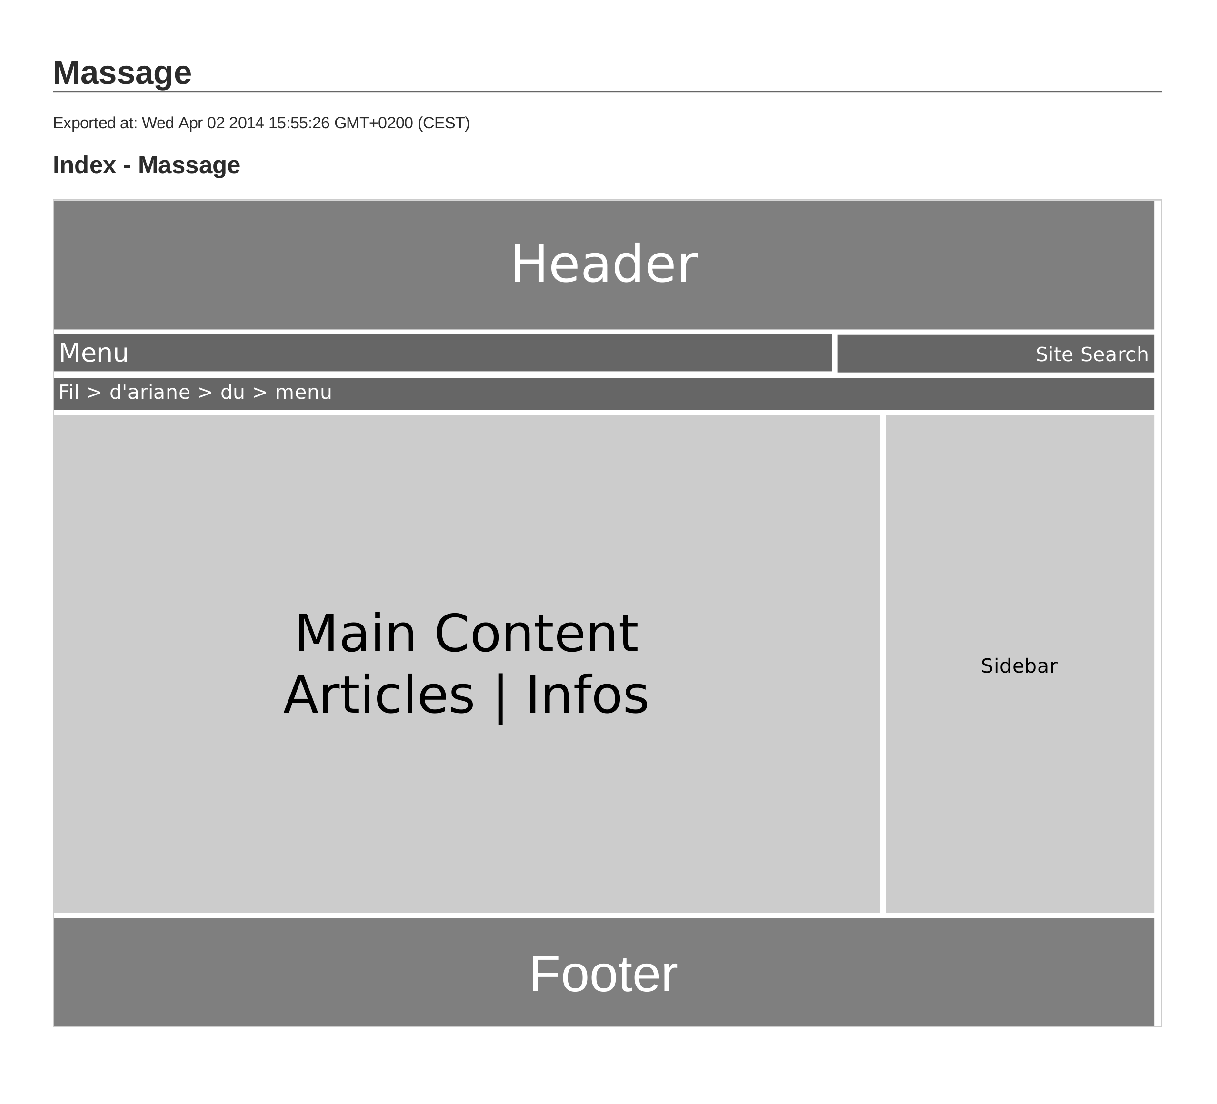
\includegraphics[height=10cm]{Zone-Massage.eps}
					\caption{Exemple de Zoning pour le site "Massage"}
					\label{fig:Zoning Massage}
				\end{figure}
				\begin{figure}[H]
					\centering
					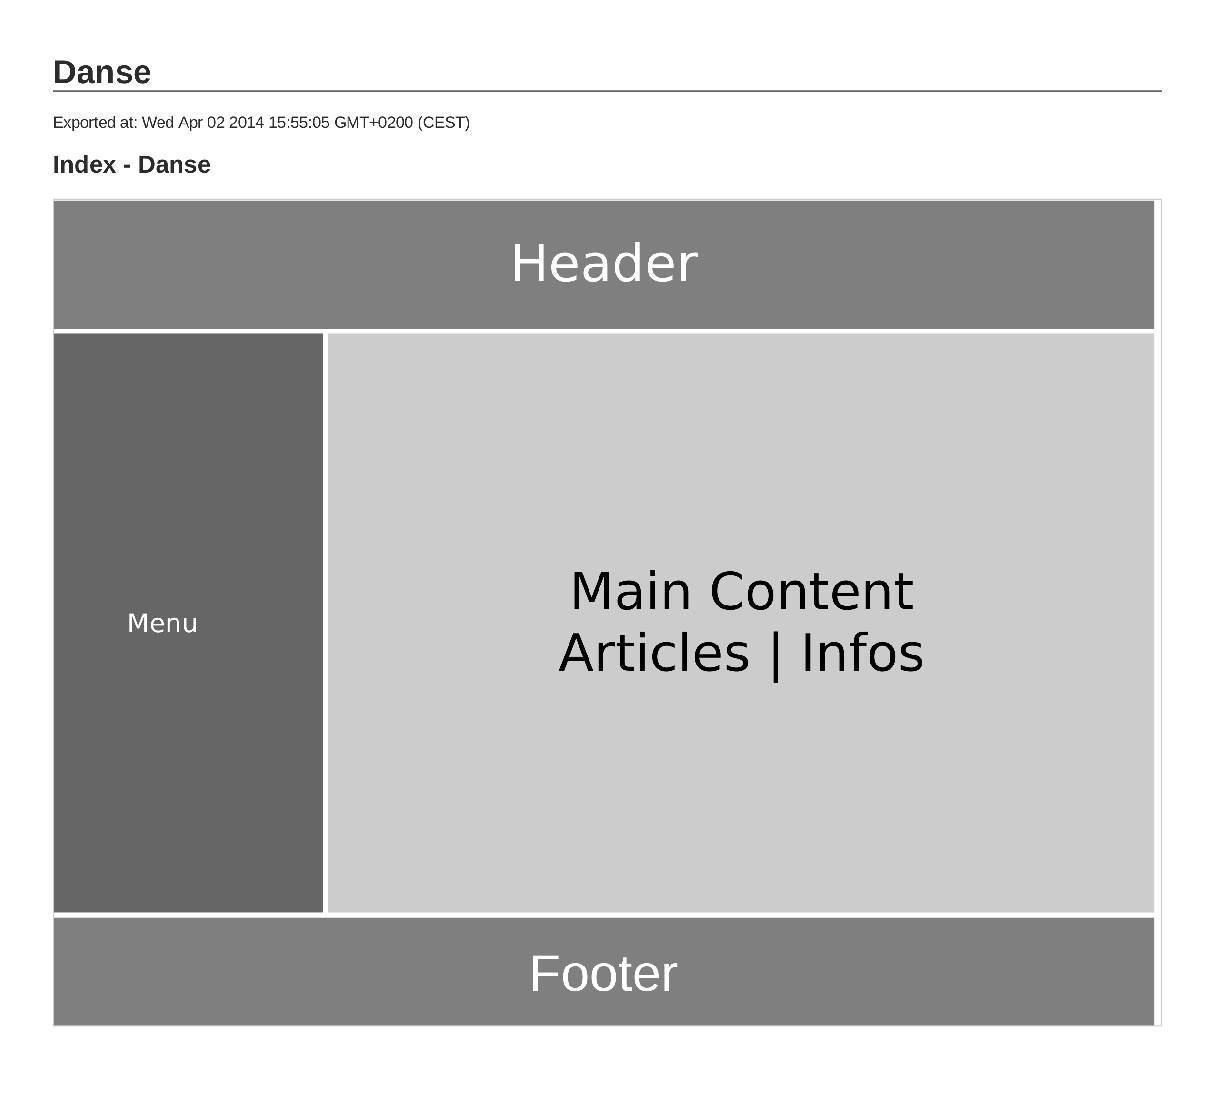
\includegraphics[height=10cm]{Zone-Danse.eps}
					\caption{Exemple de Zoning pour le site "Danse"}
					\label{fig:Zoning Danse}
				\end{figure}

			\paragraph*{Wireframe}J'ai ensuite préparé des Wireframes pour présenter les différentes possibilités offertes lors de la réalisation des sites. À ce moment là, le périmètre de l'application n'avais pas encore été défini, j'ai donc utilisé ces présentations pour expliquer les différents choix possible de réalisation.

				\begin{figure}[H]
					\centering
					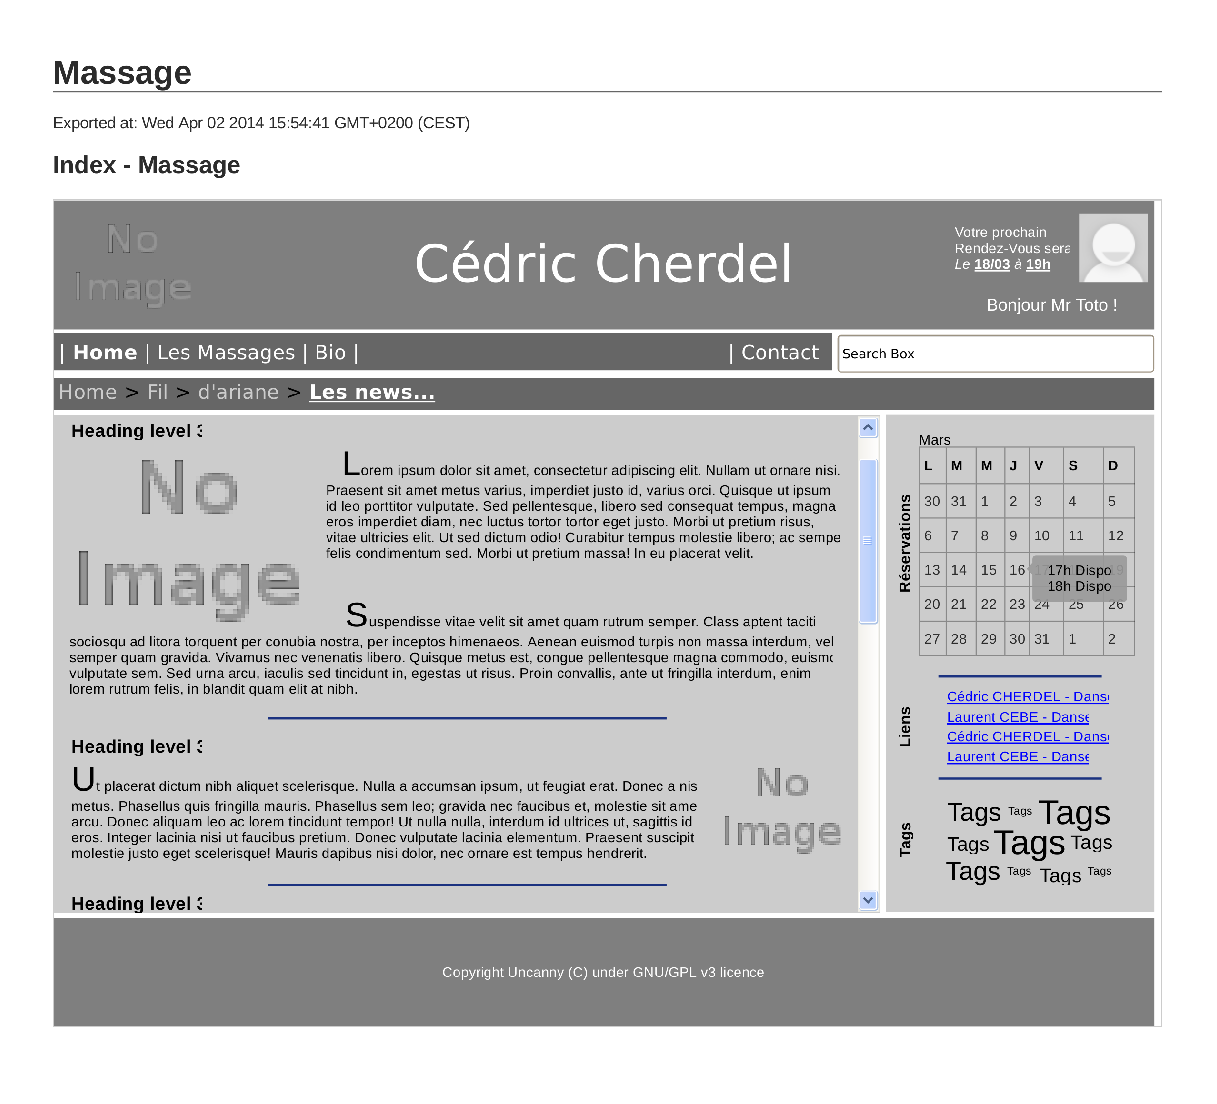
\includegraphics[height=10cm]{Wireframe-Massage_1.eps}
					\caption{Exemple de Wireframe pour le site "Massage"}
					\label{fig:Wireframe Massage}
				\end{figure}
				\begin{figure}[H]
					\centering
					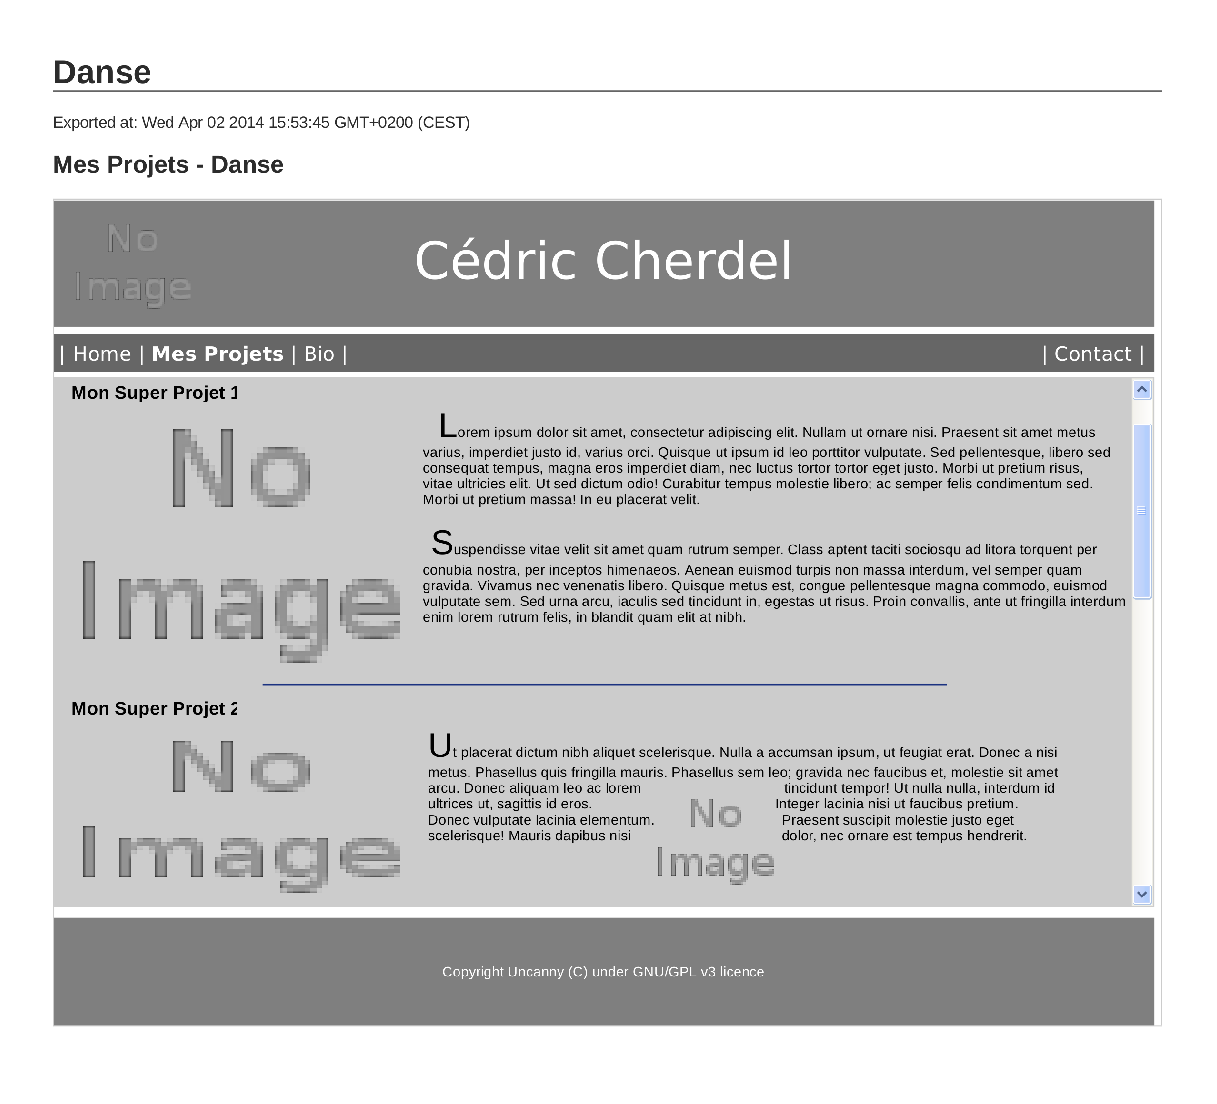
\includegraphics[height=10cm]{Wireframe-Danse_1.eps}
					\caption{Exemple de Wireframe pour le site "Danse"}
					\label{fig:Wireframe Danse}
				\end{figure}

			\paragraph*{Prototype}J'ai ensuite réalisé un prototype avec Wordpress pour présenter les différents développements requis avec Wordpress, et les contraintes liée à ce CMS. Ce prototype m'as permis de mettre en place sur un serveur de test Wordpress, MySQL ainsi que PHP5. J'en ai profité pour commencer à développer le thème des sites pour Wordpress.

				\begin{figure}[H]
					\centering
					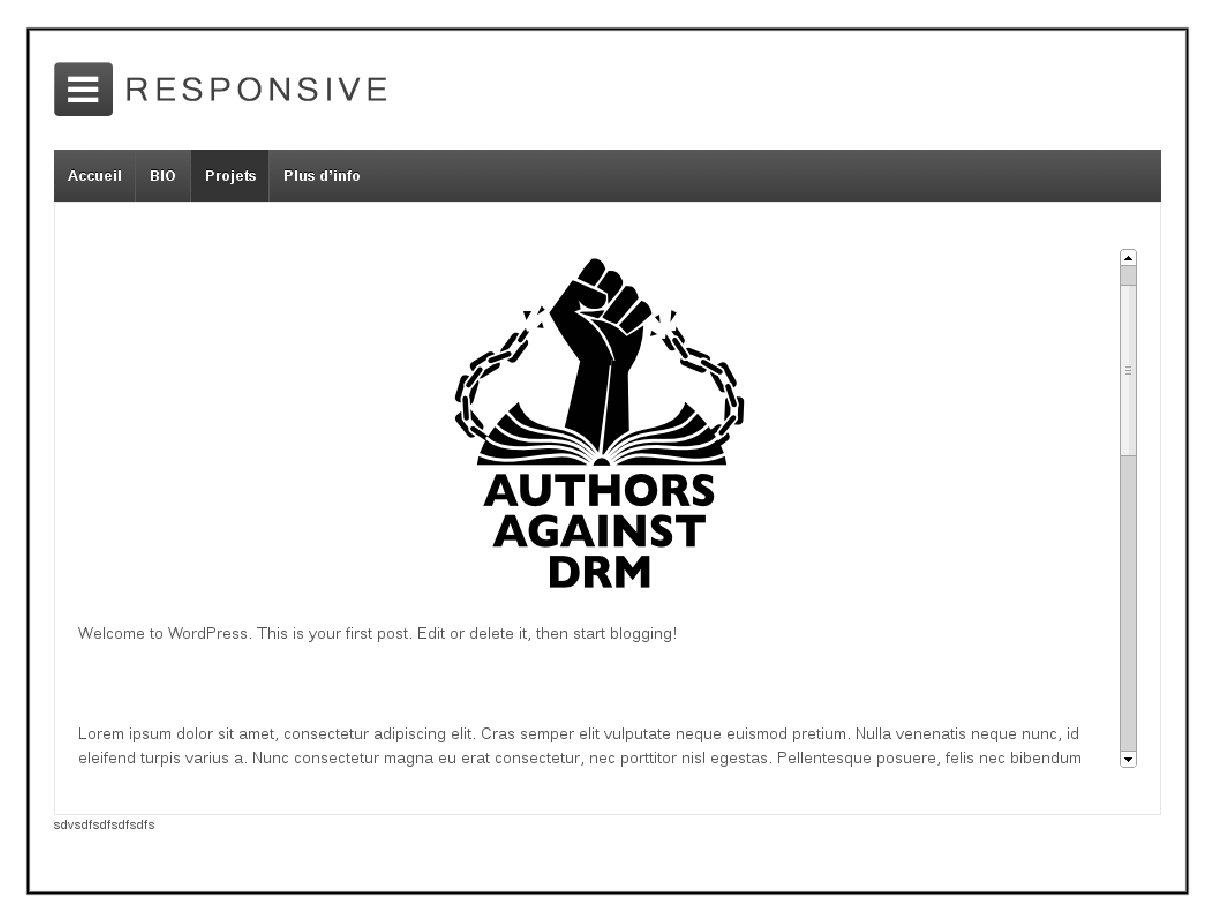
\includegraphics[height=10cm]{Prototype.eps}
					\caption{Prototype présenté pour validation}
					\label{fig:Prototype}
				\end{figure}

			\paragraph*{Styles Tiles \& Mockup}De son coté, Laurent Cebe, a réalisé des mokups et a commencé à travailler sur les styles tiles et la charte graphique.

				\begin{figure}[H]
					\centering
					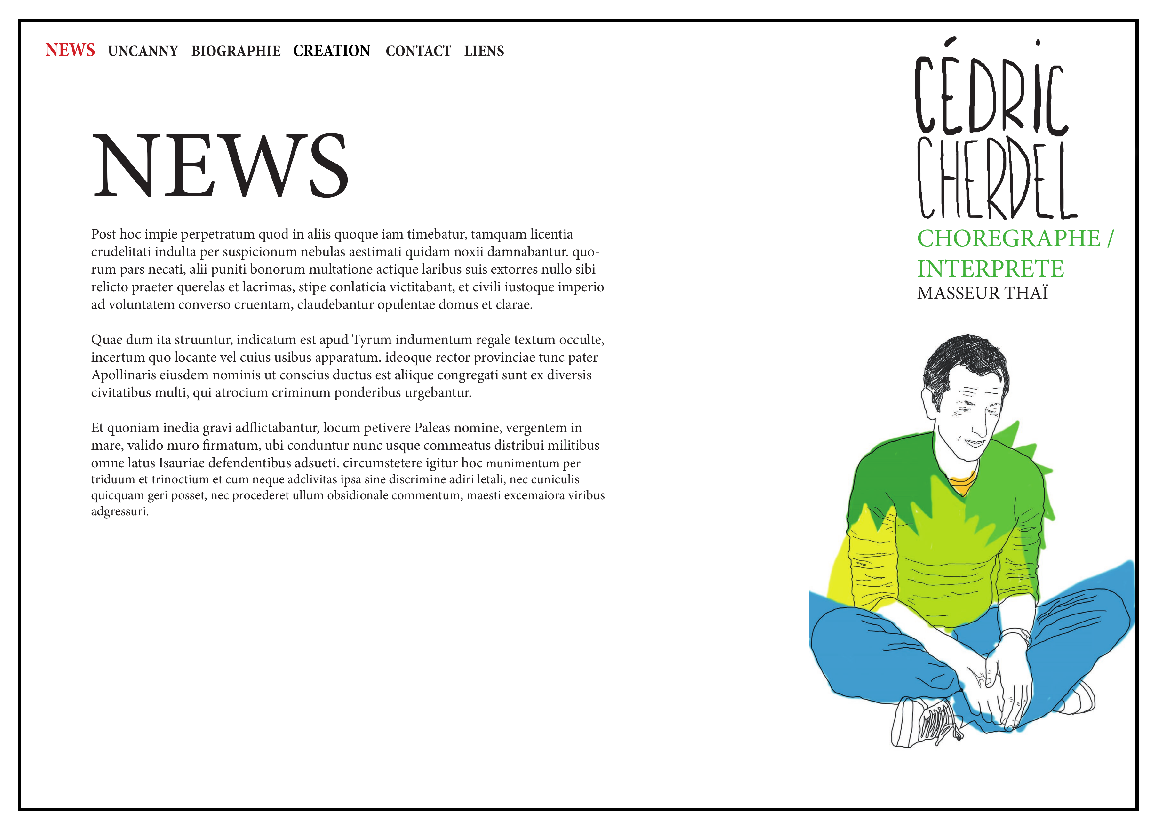
\includegraphics[height=10cm]{Mockup-Danse_1.eps}
					\caption{Mockup page d'accueil du site "Danse"}
					\label{fig:Mockup Danse Accueil}
				\end{figure}
				\begin{figure}[H]
					\centering
					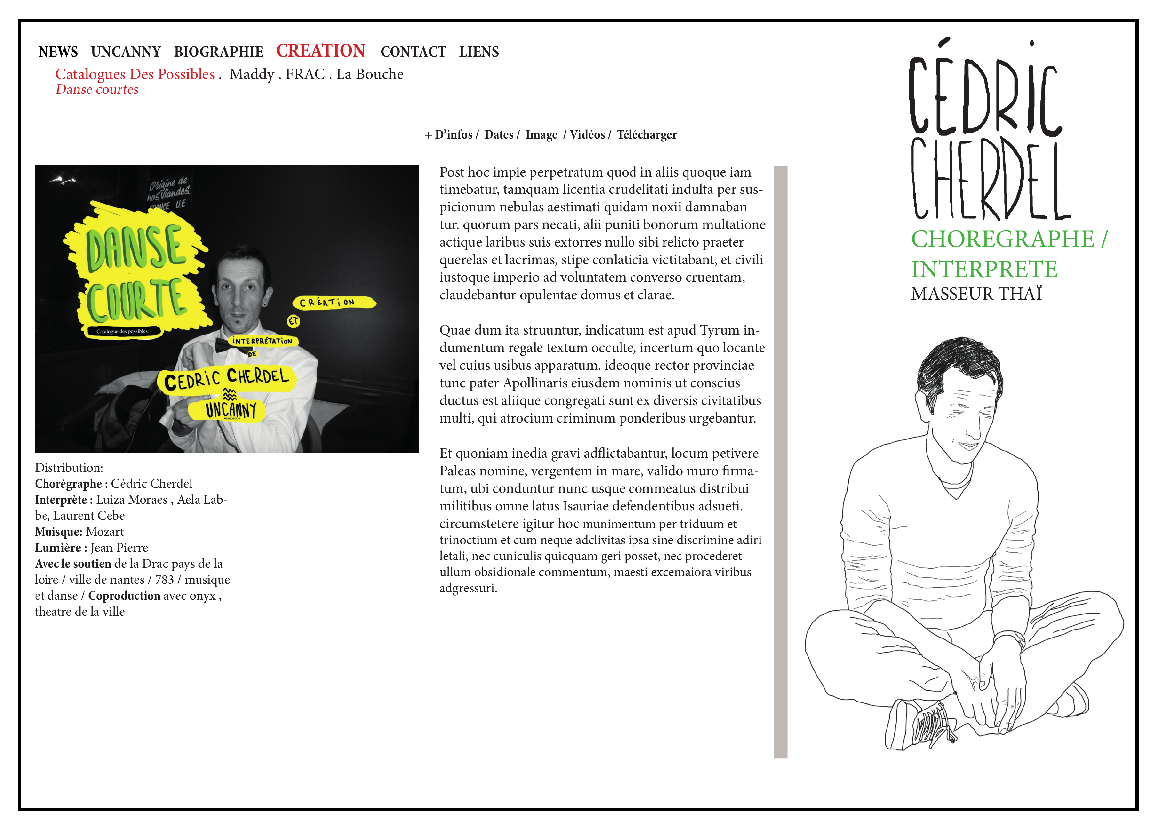
\includegraphics[height=10cm]{Mockup-Danse_2.eps}
					\caption{Mockup page projets du site "Danse"}
					\label{fig:Mockup Danse Projet}
				\end{figure}\newpage

	\section{Planning: méthodes et outils}
		\subsection{Cahier des charges}
			\paragraph*{}J'ai commencé par rédiger un premier cahier des charges vierge (basé sur un modèle fournie par l'I.M.I.E.). Lors du premier jours, j'ai expliqué rapidement l'utilité d'un CDC, puis dans une deuxième réunion, nous avons échangé autour des questions destinées à remplir ce document. Enfin, lors de la réunion de validation, nous avons repris tout les points afin de les valider. Vous le trouverez en annexe 6.
			\paragraph*{}En parallèle du CDC, j'ai réalisé un petit comparatif, sous forme de tableau, de trois offre d'hébergement pour ce projet. A savoir, 1\&1\footnote{\url{http://www.1and1.fr/}}, OVH\footnote{\url{http://www.ovh.com/fr/index.xml}} et Gandi.net\footnote{\url{https://www.gandi.net/}}. Le voici:\\

				\begin{center}
					\begin{tabular}{|l|c|c|c|}
						\hline  & Gandi.net & OVH & 1\&1 \\ 
						\hline Domaine (\euro{} HT)\cellcolor[gray]{0.9} & \cellcolor[gray]{0.9} & \cellcolor[gray]{0.9} & \cellcolor[gray]{0.9} \\ 
						.fr & 12,00\euro{} & 6,99\euro{} & 9,99\euro{} \\ 
						.com & 12,54\euro{} & 6,99\euro{} & 9,99\euro{} \\ 
						.danse & 18,80\euro{} & -- & -- \\ 
						\hline Hébergement\cellcolor[gray]{0.9} & \cellcolor[gray]{0.9} & \cellcolor[gray]{0.9} & \cellcolor[gray]{0.9} \\ 
						Disque & 10Go & 100Go & 50Go \\ 
						Quota (Go/mois) & 60Go & Illimité & ? \\ 
						Bases SQL & illimités & 1x 200Mo & 1x 1Go \\
						Versionning  & Git & -- & -- \\ 
						Upload & sftp & ftp & ftp \\ 
						Shell & ssh & -- & -- \\ 
						Mail & 5x 1Go & 10x 5Go & ? \\ 
						Hébergement (\euro{} HT)\cellcolor[gray]{0.9} & 48,00\euro{}\cellcolor[gray]{0.9} & 23,88\euro{}\cellcolor[gray]{0.9} & 35,88\euro{}\cellcolor[gray]{0.9} \\ 
						Total .com + Hébergement (TTC)\cellcolor[gray]{0.7} & 72,65\euro{}\cellcolor[gray]{0.7} & 37,04\euro{}\cellcolor[gray]{0.7} & 55,04\euro{}\cellcolor[gray]{0.7} \\ 
						\hline 
					\end{tabular}
				\end{center}

			\paragraph*{}Le choix, au vu des ces éléments et des fonds disponibles, c'est porté sur OVH. Malheureusement pour nous, ce dernier ne permet pas d'installer des scriptes Ruby et de les lancer via des taches "cron" de façon régulière, nous allons donc mettre en place sur une machine locale, tout les éléments nécessaires pour ce projet. Il à été choisi par le client que dès l'arrivée de fonds supplémentaires, nous basculerons sur une offre Gandi qui apporte ces fonctionnalités.
			\newpage
		\subsection{Pert \& Gantt}
			\paragraph*{Prévisionnel}Les Pert et Gantt sont réalisé avec Planner\footnote{\url{http://live.gnome.org/Planner} : application Gnome en GNU/GPL v2}.
			\paragraph*{}J'ai commencé par ajouter les actions ainsi que les jalons dans Planner et j'ai estimé la charge de travail. Lors de ce projet, j'ai utilisé deux versions de mon Gantt, un Gantt prévisionnel (réalisé en début de projet) et un Gantt réel (avec une mise à jours des dates de validations en fonction des vrais dates de rendez-vous)

				\begin{figure}[H]
					\centering
					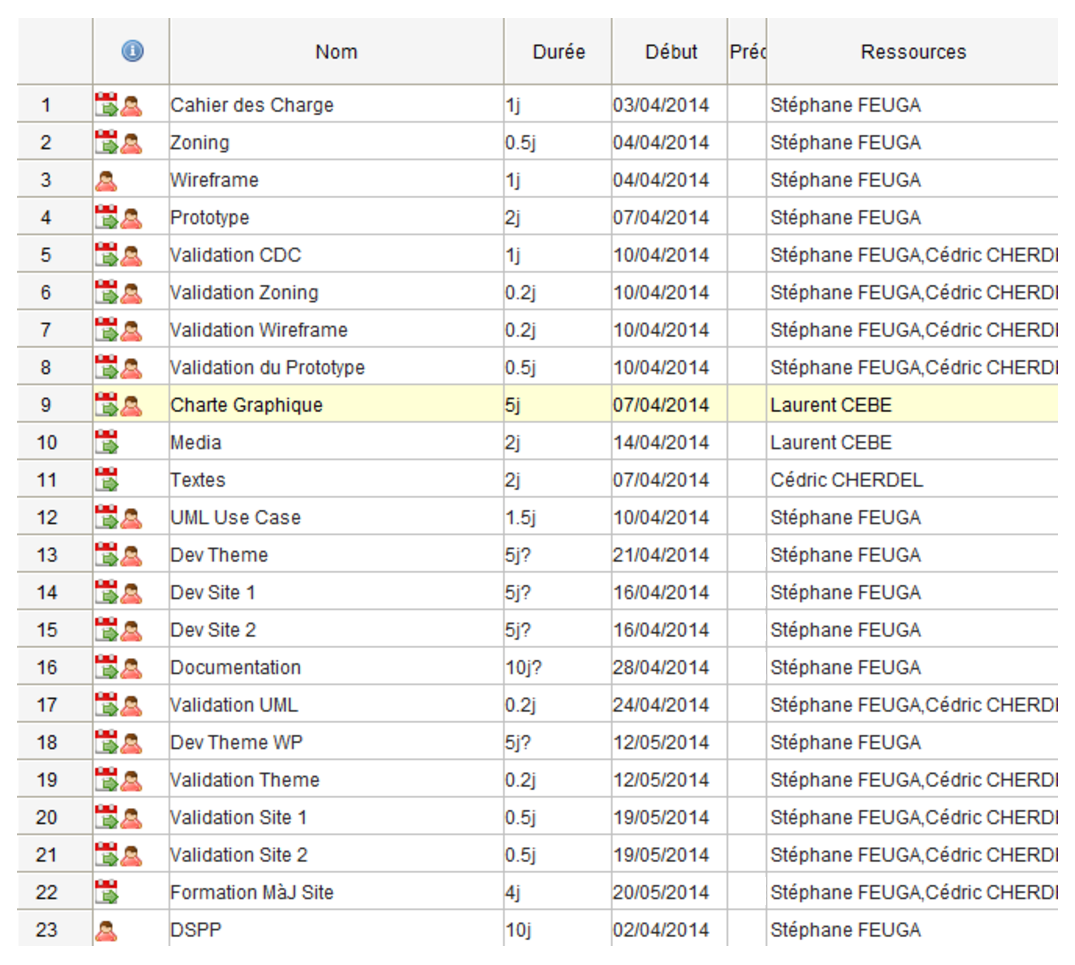
\includegraphics[height=10cm]{Gantt_Previsionnel_1.eps}
					\caption{Liste des actions et des Jalons}
					\label{fig:List des Actions Gantt Previsionnel}
				\end{figure}\newpage
			\paragraph*{}Puis j'ai lié les éléments avec leurs prédécesseurs, ce qui donne le graphique suivant: 

				\begin{figure}[H]
					\centering
					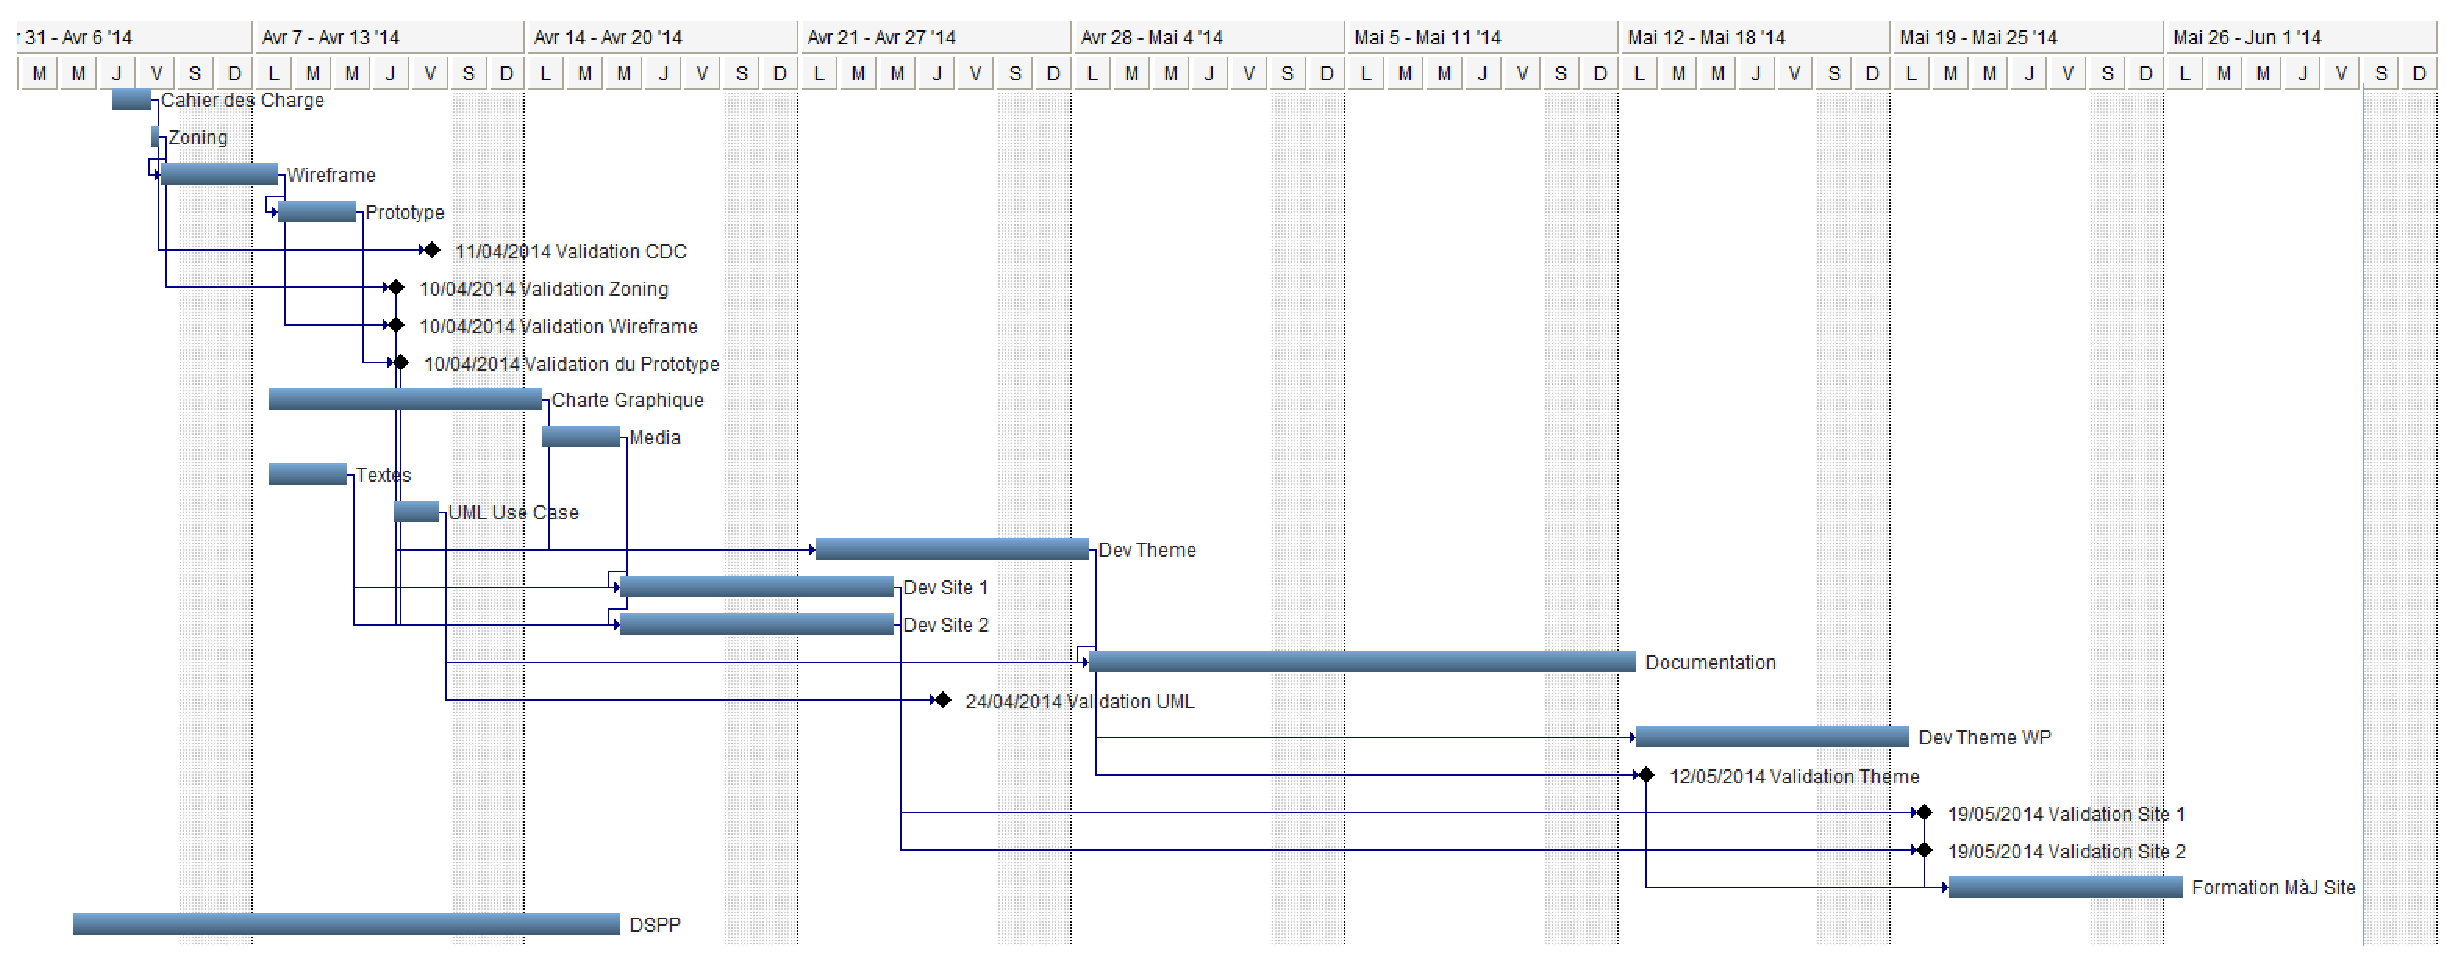
\includegraphics[width=\textwidth]{Gantt_Previsionnel_2.eps}
					\caption{Gantt prévisionnel fini}
					\label{fig:Graphique Gantt Previsionnel}
				\end{figure}
			\paragraph*{Réel}Enfin, j'ai dupliqué ce Gantt et je l'ai modifié en fonction des dates de validations réels. En voici le résultat: 

				\begin{figure}[H]
					\centering
					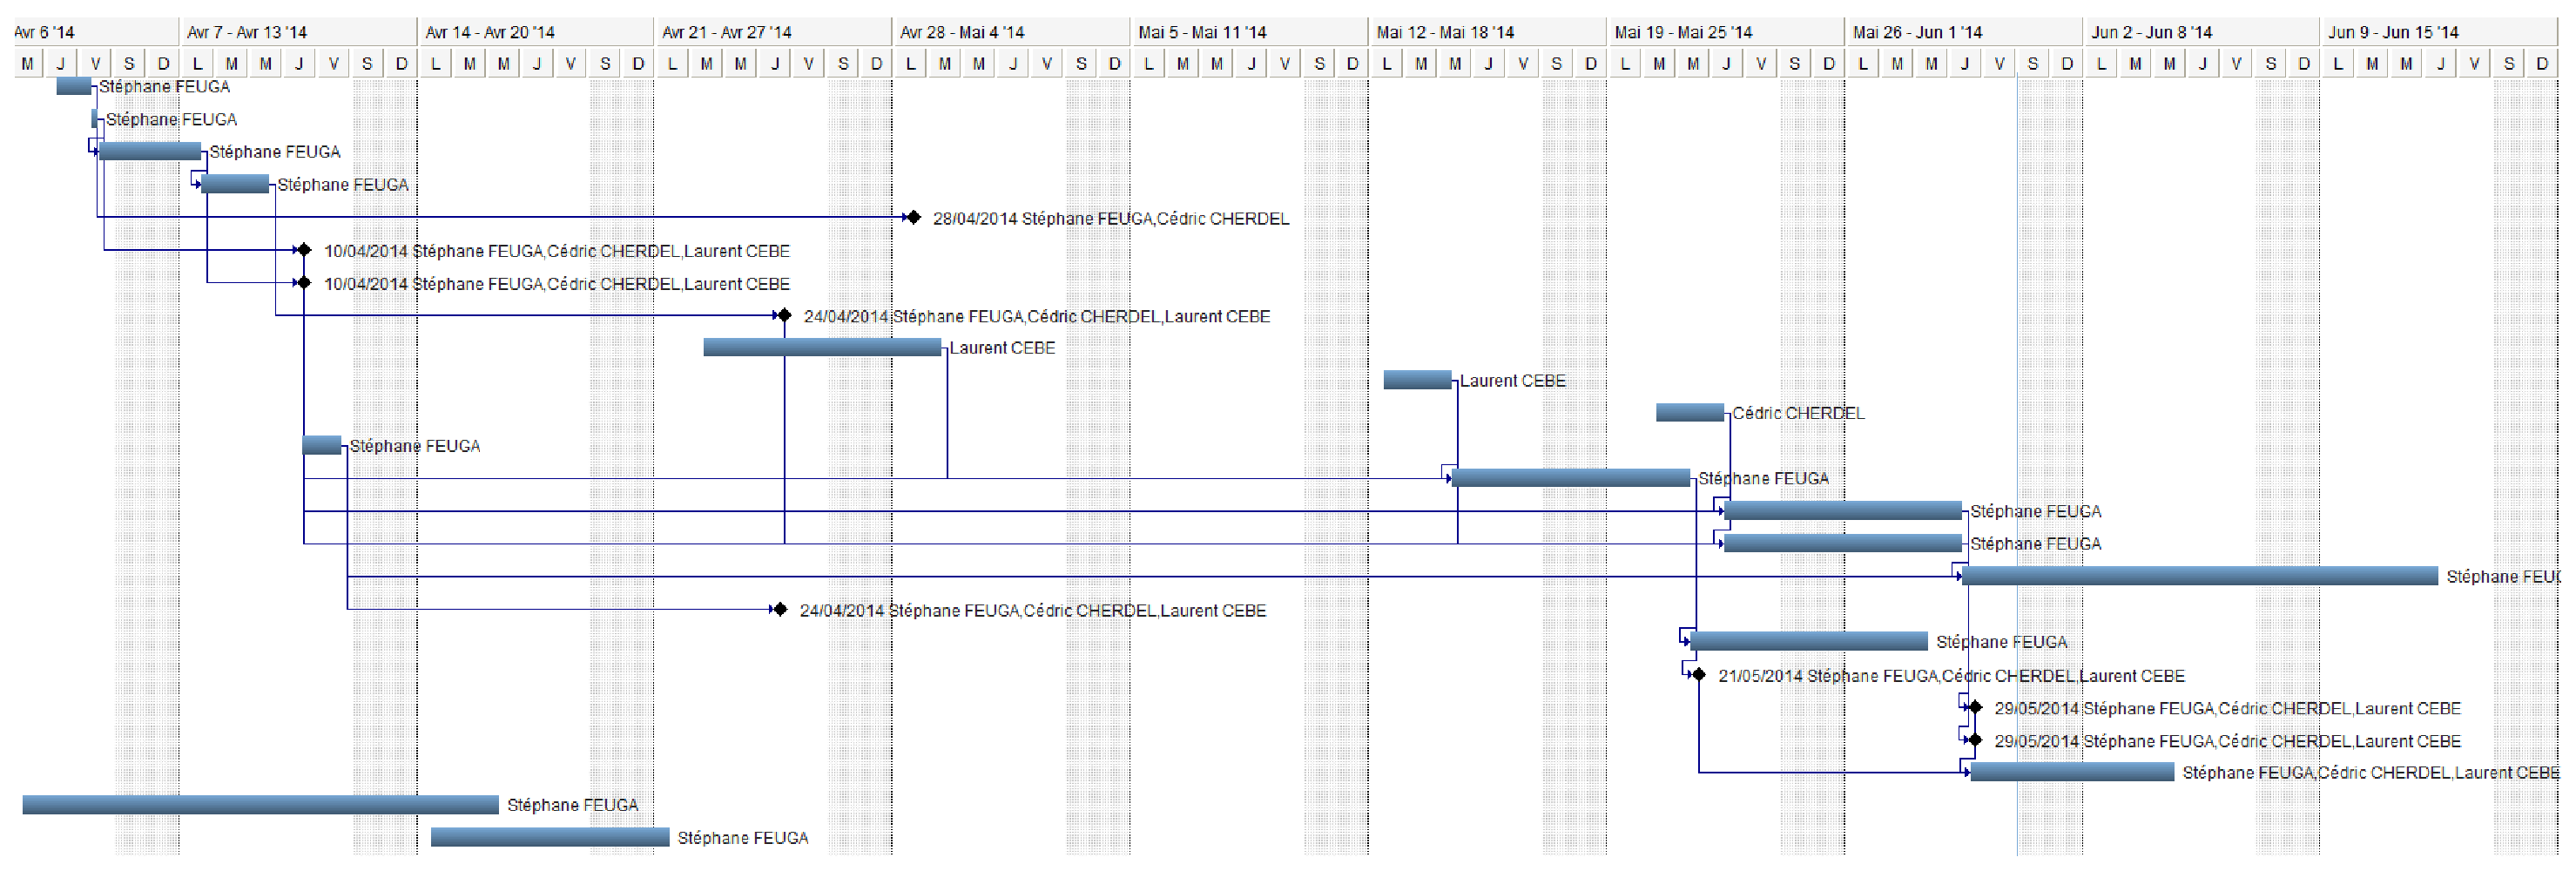
\includegraphics[width=\textwidth]{Gantt_Reel_2.eps}
					\caption{Gantt prévisionnel fini}
					\label{fig:Gantt Reel}
				\end{figure}
				\subparagraph*{}Les principaux problèmes de planning rencontrés lors de ce stage sont lié au manque de disponibilité de Cédric et Laurent. Pendant cette période, ils se sont attelé à mettre en scène un nouveau spectacle qui sera présenté les 25 et 26 Juin prochains. J'ai du mettre certaines action en \textit{"pause"} le temps d'avoir des réponses et validations attendu. J'ai mis ce temps de \textit{"disponibilité"} à profits en me formant aux bases de Ruby on Rails pour JekyllRB. J'ai aussi eu du temps pour me documenter sur la danse contemporaine et sur les différentes techniques de massage Thaï.
				\subparagraph*{}J'ai aussi passé beaucoup de temps à préparer les éléments graphiques et à travailler sur la charte graphique car par manque de temps, Laurent n'as pas pu exécuter tout ce qu'il souhaitait faire.
				\newpage

		\subsection{Agilité, Scrum Board \& Git}
			\paragraph*{}Nous avons choisi de travailler en Agilité. Les Sprints sont d'une semaine et ne se rapport qu'à une fonctionnalité. Nous utilisons intensivement un Scrum Board\footnote{\url{http://tsu3d.hestia.feralhosting.com/scrum}}.
			\paragraph*{}Ce mode de fonctionnement m'as permis d'avoir un grande réactivité lors de changement important et l'utilisation d'un Scrum Board à permis à toutes les parties prenantes de suivre l'avancement du projet au jour le jour.
			Le Scrum board est réalisé en PHP, jQuery et HTML5. La base de données est en SQLite. C'est un fork réalisé depuis le projet kanboard\footnote{\url{https://github.com/fguillot/kanboard}} et modifié par mes soins.
			\begin{figure}[H]
				\centering
				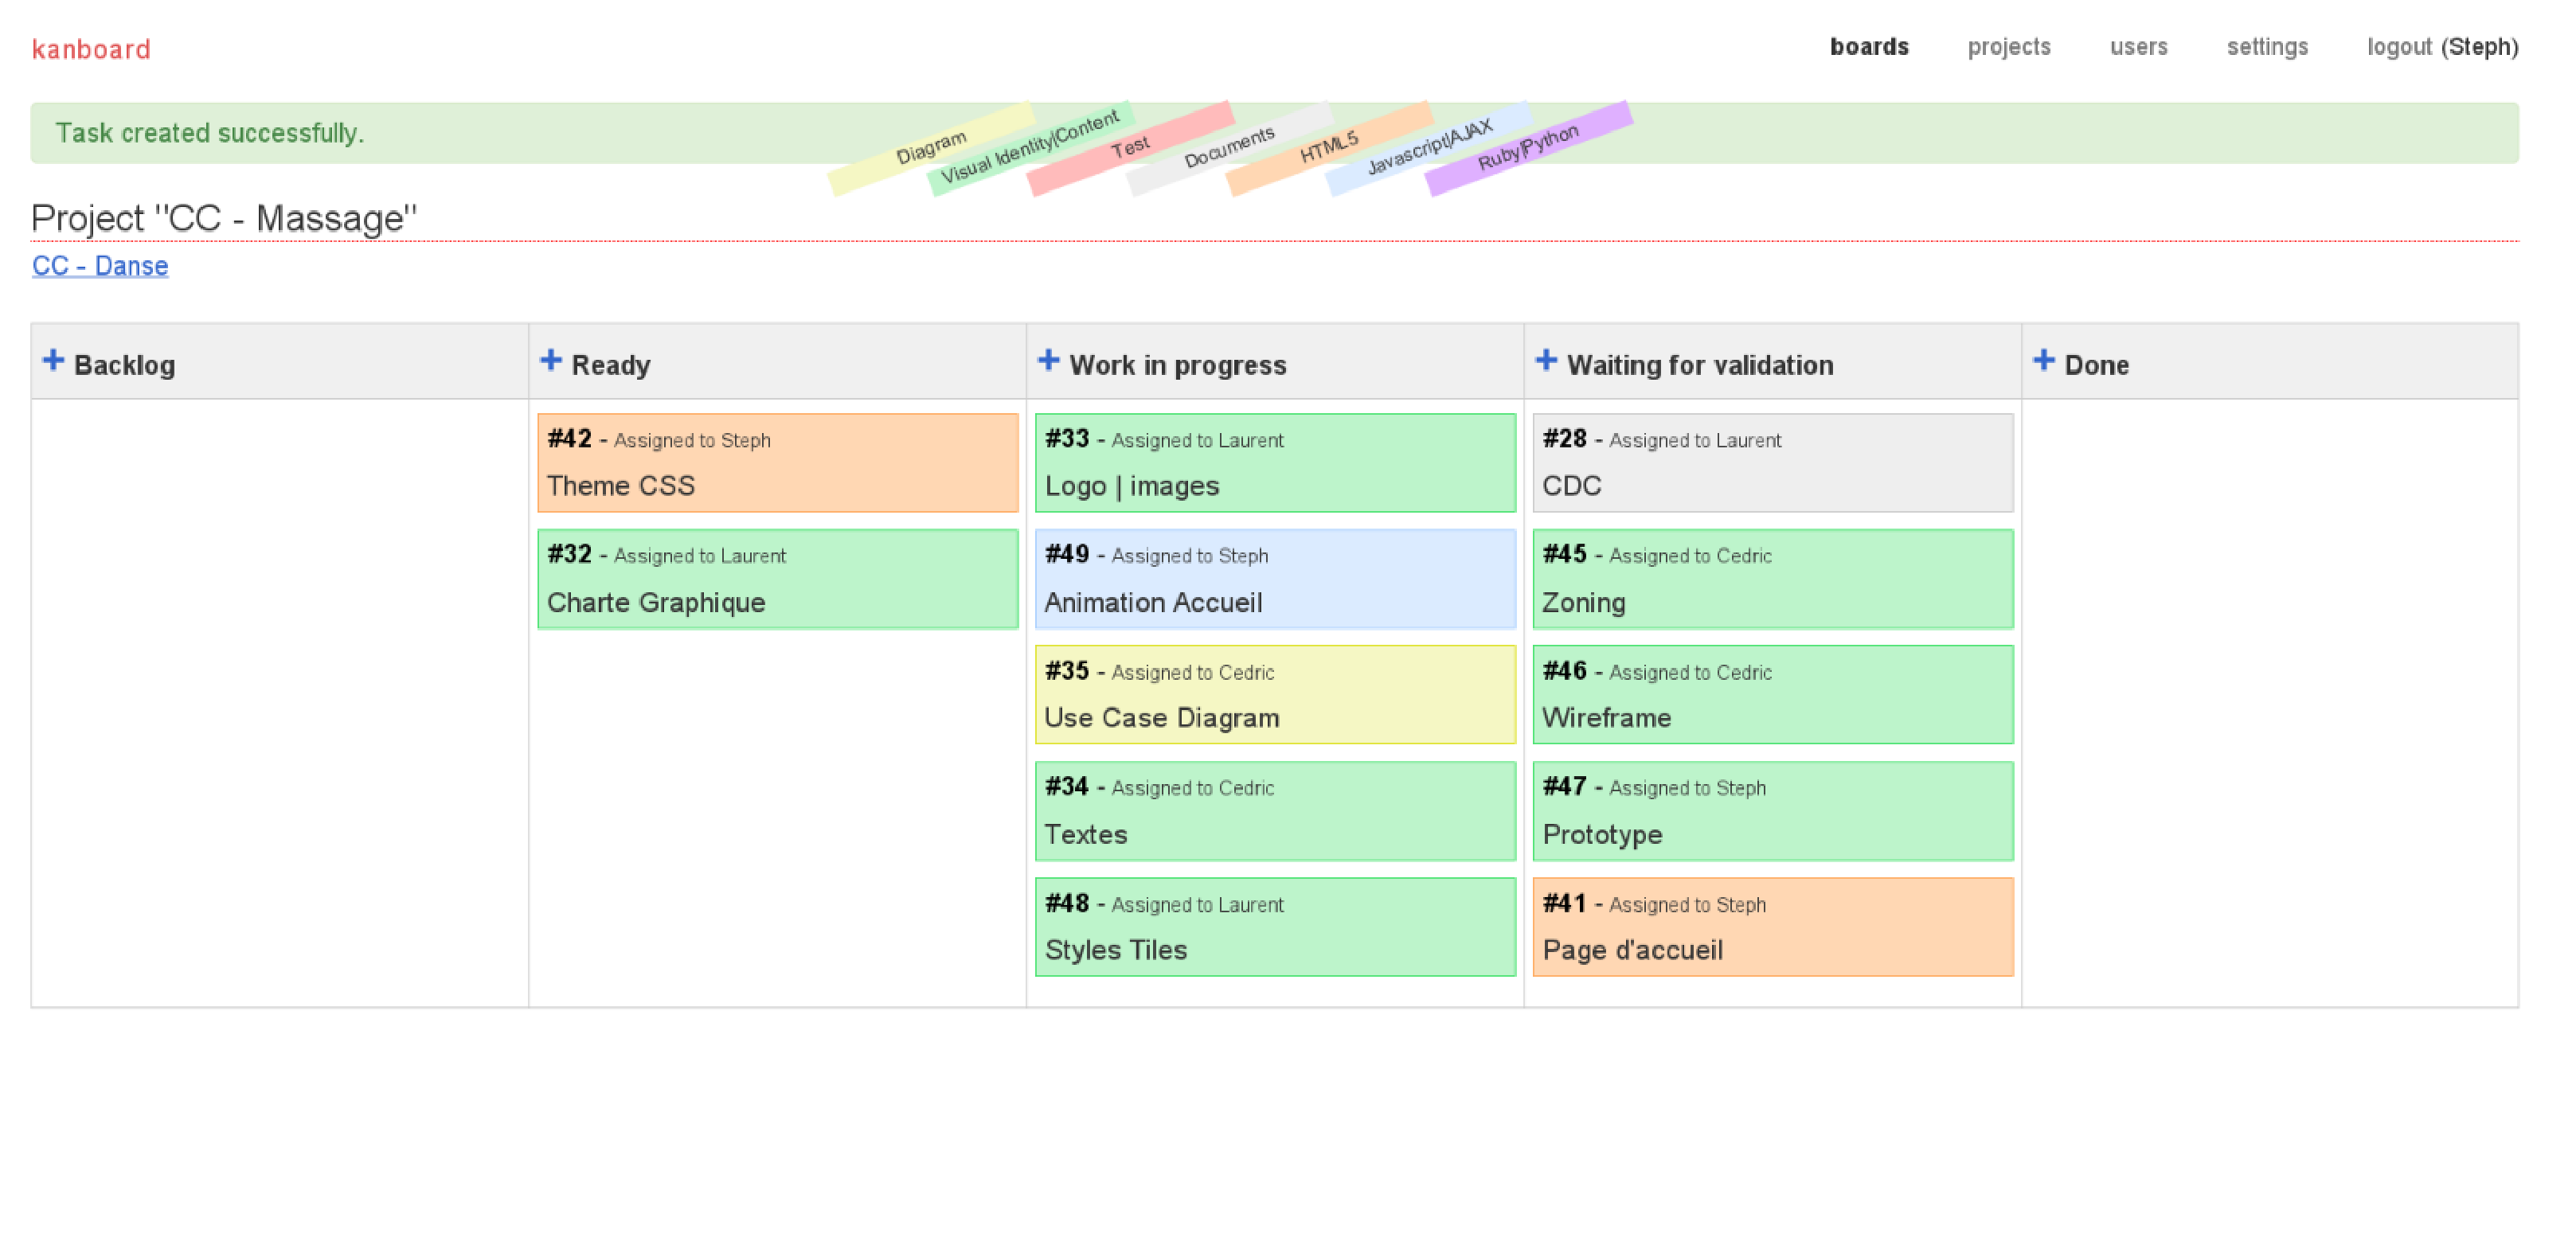
\includegraphics[width=\textwidth]{kanban1.eps}
				\caption[Kanban Board]{Exemple d'utilisation du Scrum Board pour le site "Massage"}
				\label{fig:Kanban Board}
			\end{figure}
			\newpage
			\begin{figure}[H]
				\centering
				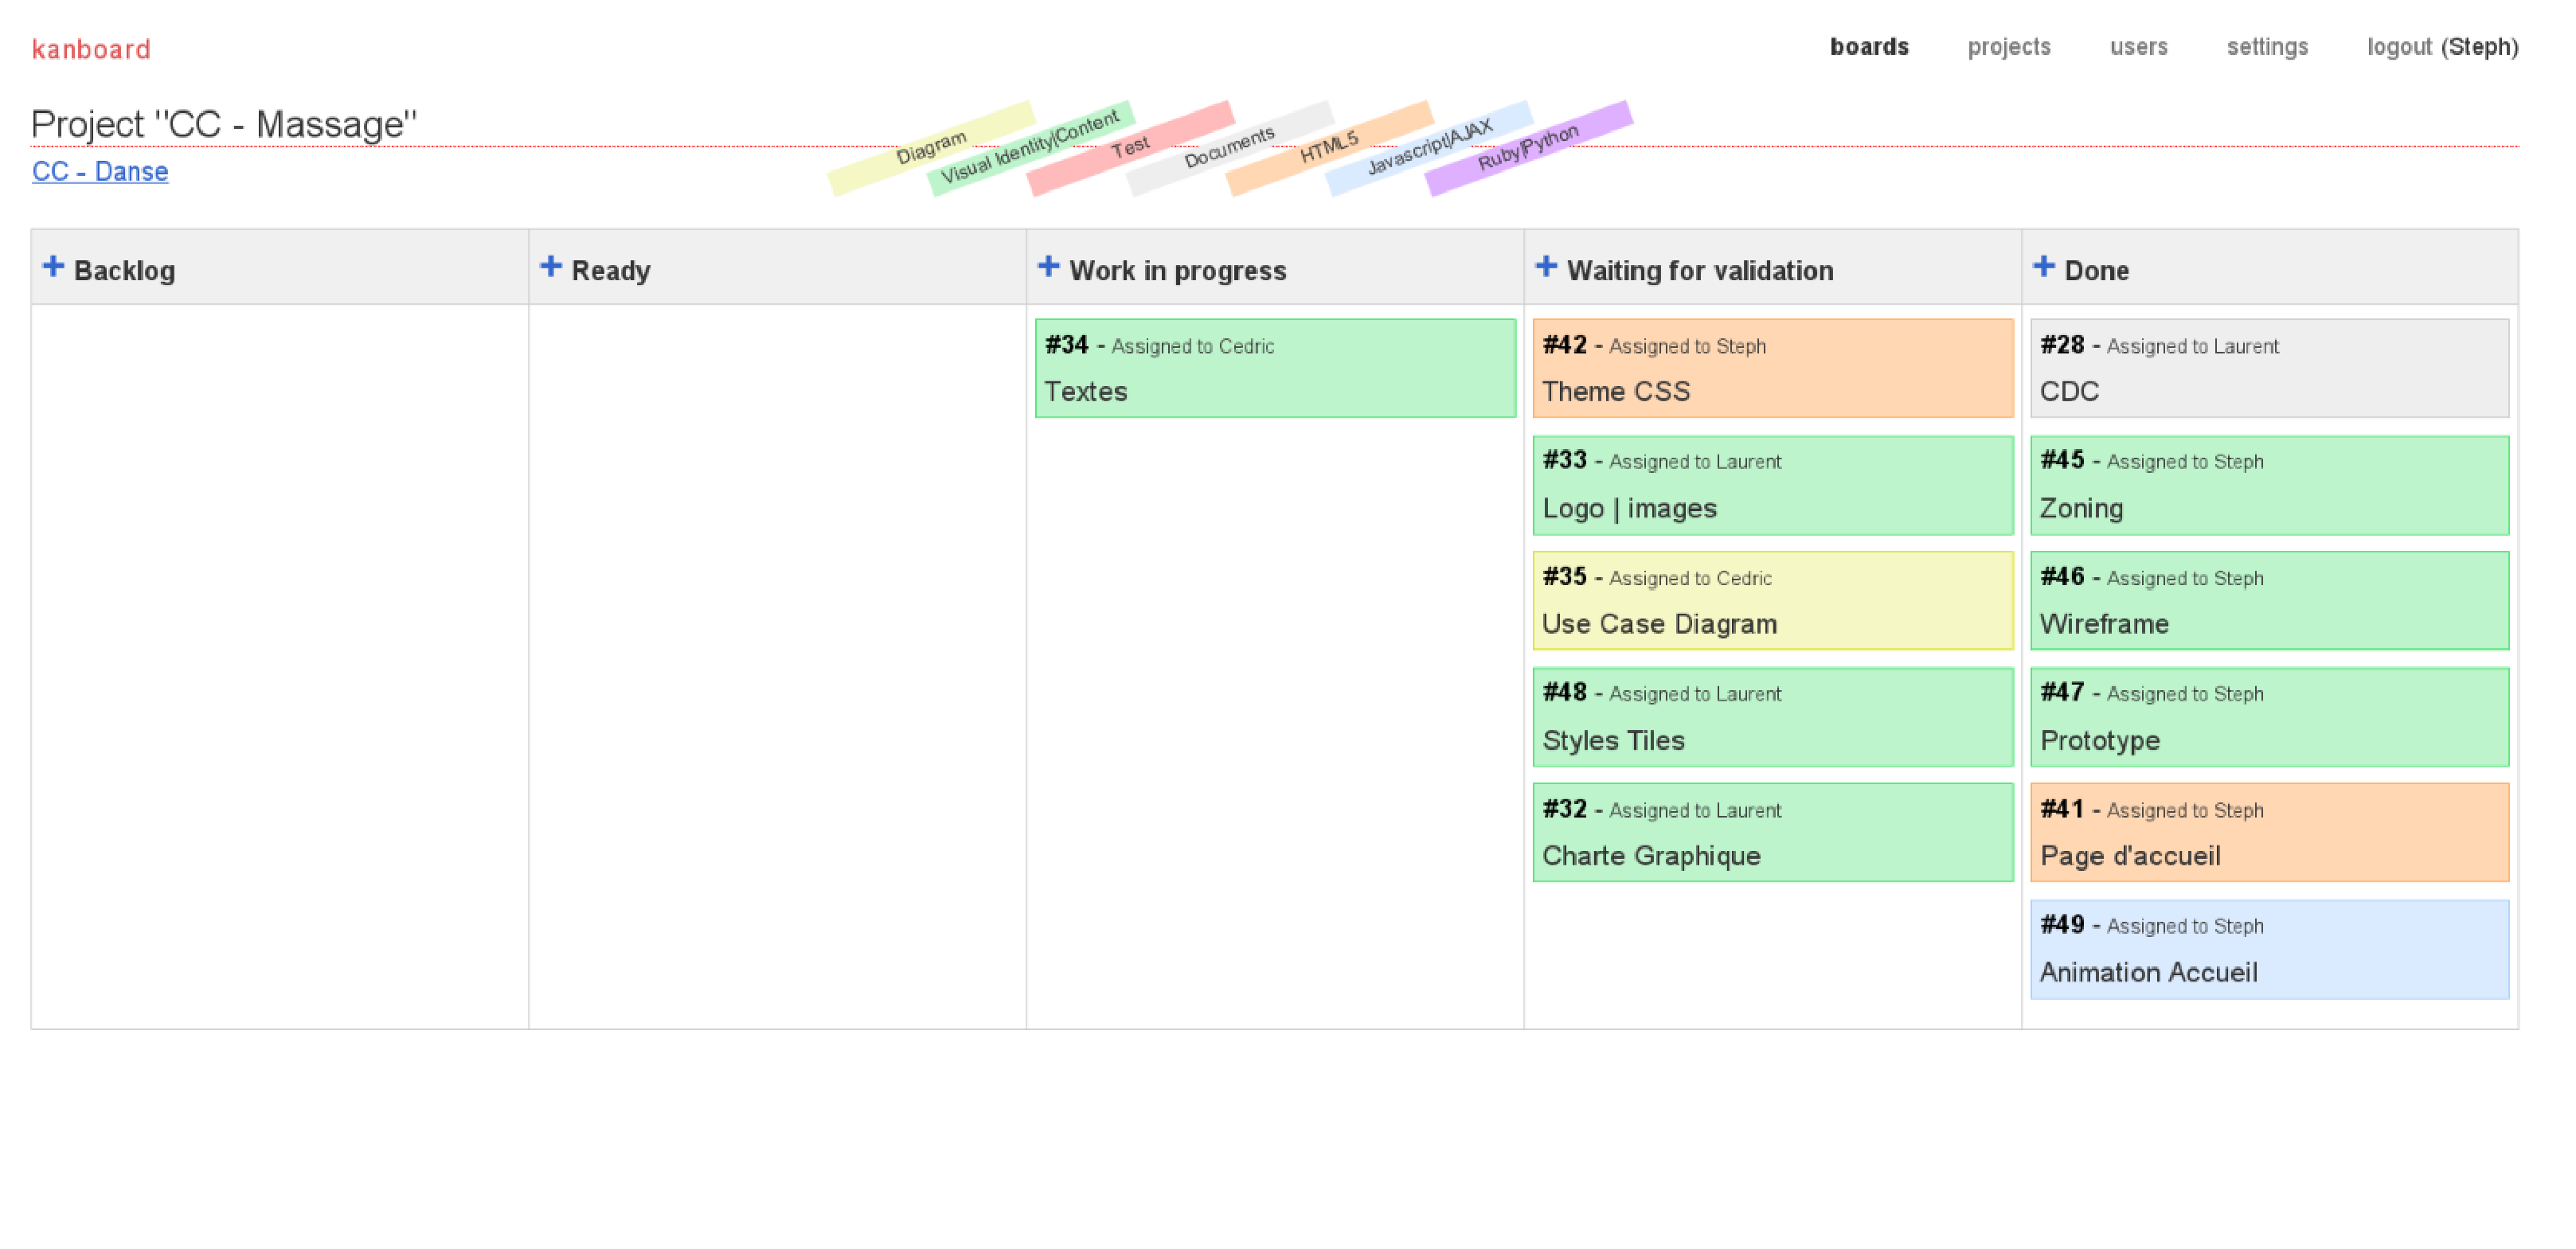
\includegraphics[width=\textwidth]{kanban2.eps}
				\caption[Kanban Board]{Scrum Board du site "Massage" Mis à Jour}
				\label{fig:Kanban Board v2}
			\end{figure}
			\paragraph*{}Le choix du gestionnaire de version à été rapide, j'utilise depuis fin 2005 GIT. Nous avons aussi choisi Gitorious\footnote{\url{https://gitorious.org/uncanny}} comme plateforme d'hébergement car tout son code source est sous licence GNU/AGPL v3. L'utilisation de GIT fut intensive. Plusieurs \textit{"Repository"} ont été créé pour partager (et garder une trace des modifications) aussi bien les différents codes sources des sites, que les documentations, le cahier des charges (et ses annexes) ainsi que ce rapport. Ça a permis à tout le monde d'avoir accès à tout et de pouvoir en suivre les modifications.\\
			Les différents répertoires sont:
				\begin{itemize}
					\item \textbf{theme}: Thème Wordpress (en cours de développement pour évolution futur).
					\item \textbf{site\_massage}: Site Massage sous Wordpress (en cours de développement pour évolution futur).
					\item \textbf{site\_danse}: Site Danse sous Wordpress (en cours de développement pour évolution futur).
					\item \textbf{site\_accueil}: Page d'accueil des deux sites (Réalisé en HTML5 et jQuery).
					\item \textbf{rapport\_de\_stage}: Ce rapport ainsi que toutes les annexes qui y sont liée.
					\item \textbf{cedriccherdel-massage}: Thème et Site réalisé avec JekyllRB.
					\item \textbf{cedriccherdel-danse}: Thème et Site réalisé avec JekyllRB.
				\end{itemize}
			\paragraph*{}À la suite de ce stage, il est prévu que je développe les fonctions manquantes à Wordpress pour ce projet. En effet, un des besoins exprimés au fil des rendez-vous à été une certaine \textit{"automatisation"} de la création de contenu. La demande est la suivante: on créé un nouveau post et on ajoute dans le gestionnaire de média de Wordpress, les divers éléments liés à ce post. Ces éléments peuvent-être des pdf, des images et/ou des vidéos. Le but de cette automatisation est qu'en fonction des noms de fichiers et des noms de dossiers les contenant, tous les médias présent pour ce projet, sont automatiquement ajoutés. Il n'est donc plus nécessaire de perdre du temps en "clic/sélection/clic" pour ajouter ces éléments dans le post.

\chapter{Conception}
	\section{Modélisations UML}
			\subsection{Use Case}
				\paragraph*{}J'ai commencé la modélisation de ce projet en effectuant des Uses-cases qui ont servi de validation pour le périmètre du développement.
				\paragraph*{}Ces schémas sont assez simples, mais m'ont permis d'expliquer plus simplement les fonctionnalités demandés. Une première version, avec des fonctionnalités n'apparaissant pas sur ces schémas, contenait une authentification des utilisateurs du site massage, un système de réservation de rendez-vous en ligne, la création et l'édition de newsletter depuis les sites via un back-office prévu à cette effet.
				\paragraph*{}Lors d'une séance de brainstorming, il est apparu que la prise de rendez-vous par les clients n'était pas souhaitable car ça impliquais de maintenir un calendrier de disponibilité à jours, ce qui n'est actuellement pas le cas. Pour ce qui est de la réalisation de newsletter, nous avons mis en place des modèles d'emails réutilisable utilisant la charte graphique, ce qui a permis de ne pas développer des outils inutiles.
				\paragraph*{}Nous avons donc choisi de réaliser des sites plus simples mais répondant mieux aux besoins.
					\subparagraph*{Massage}Au départ, nous avons défini que peu de pages pour ce site, les informations importantes sont: la biographie de Cédric, une page de contact avec un moyen de s'abonner à la newsletter et une description des types de massages proposés. L'administrateur du site doit-être en mesure de modifier rapidement toutes ces informations.
						\begin{figure}[H]
							\centering
							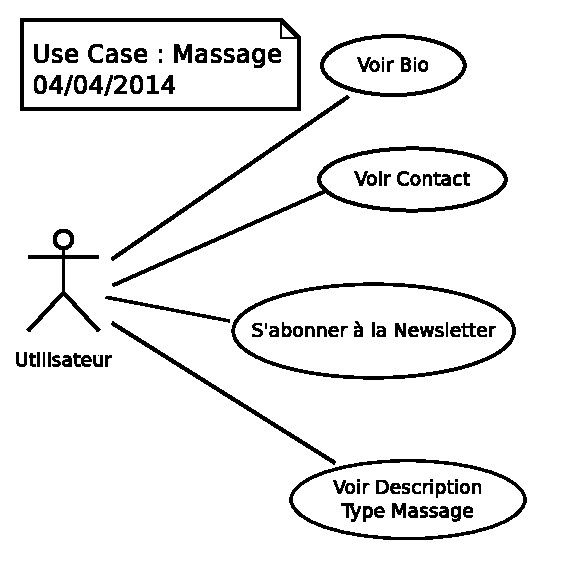
\includegraphics[width=10cm]{UseCase-Massage-User.eps}
							\caption[Use Case Utilisateur Massage]{Use Case d'un Utilisateur pour le site "Massage"}
							\label{fig:UseCase-Massage User}
						\end{figure}
						\begin{figure}[H]
							\centering
							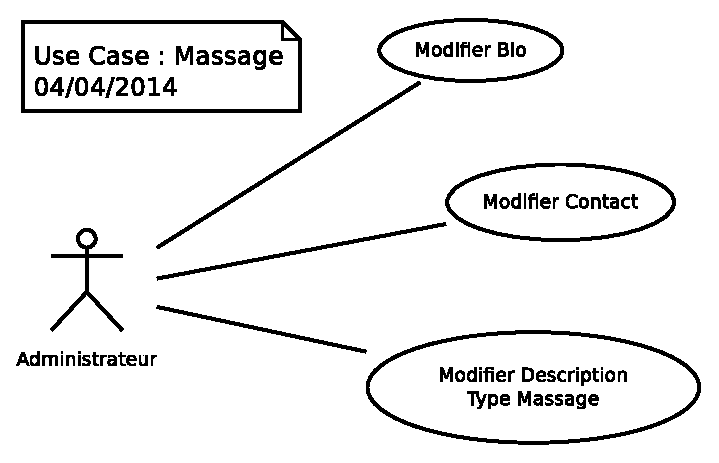
\includegraphics[width=10cm]{UseCase-Massage-Administrateur.eps}
							\caption[Use Case Administrateur Massage]{Use Case de l'administrateur pour le site "Massage"}
							\label{fig:UseCase-Massage Admin}
						\end{figure}\newpage
					\subparagraph*{Danse}Les schémas sont quasiment identiques avec l'ajout de média photos et vidéos dans les projets.
						\begin{figure}[H]
							\centering
							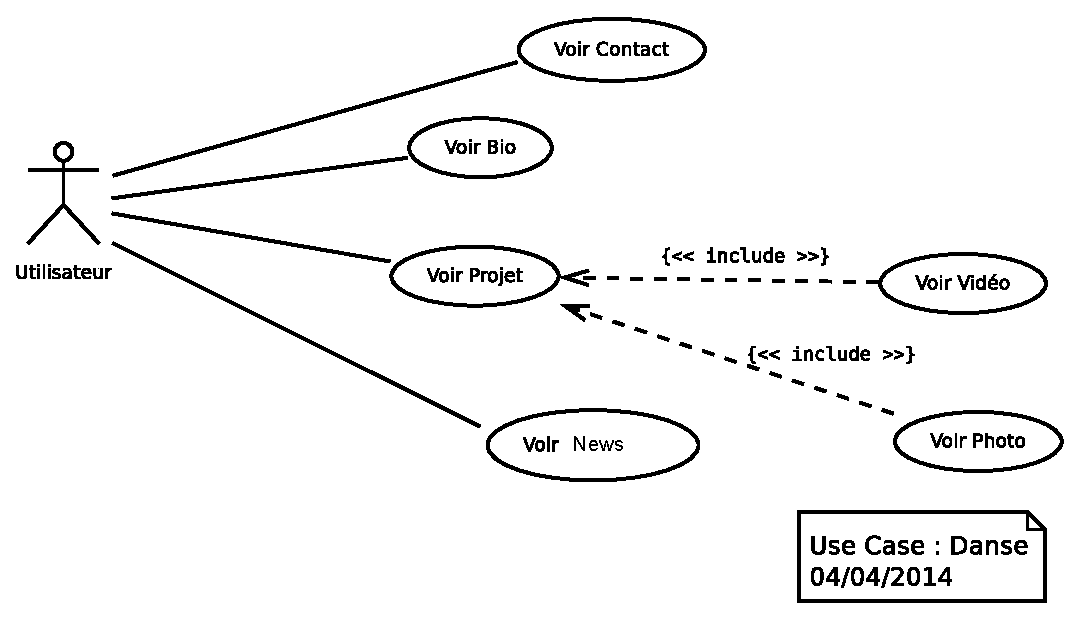
\includegraphics[width=12cm]{UseCase-Danse-User.eps}
							\caption[Use Case Utilisateur Danse]{Use Case d'un Utilisateur pour le site "Danse"}
							\label{fig:UseCase-Danse User}
						\end{figure}
						\begin{figure}[H]
							\centering
							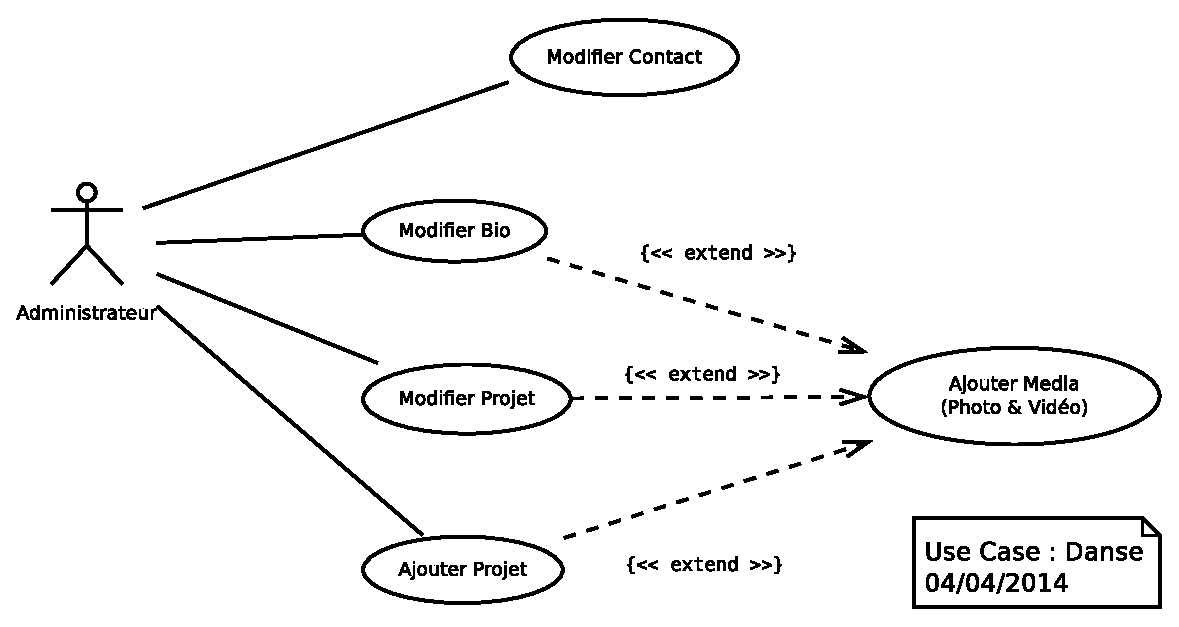
\includegraphics[width=16cm]{UseCase-Danse-Administrateur.eps}
							\caption[Use Case Administrateur Danse]{Use Case de l'administrateur pour le site "Danse"}
							\label{fig:UseCase-Danse Admin}
						\end{figure}

			\subsection{Schéma d'Enchainement des Pages Web}
				\begin{figure}[H]
					\centering
					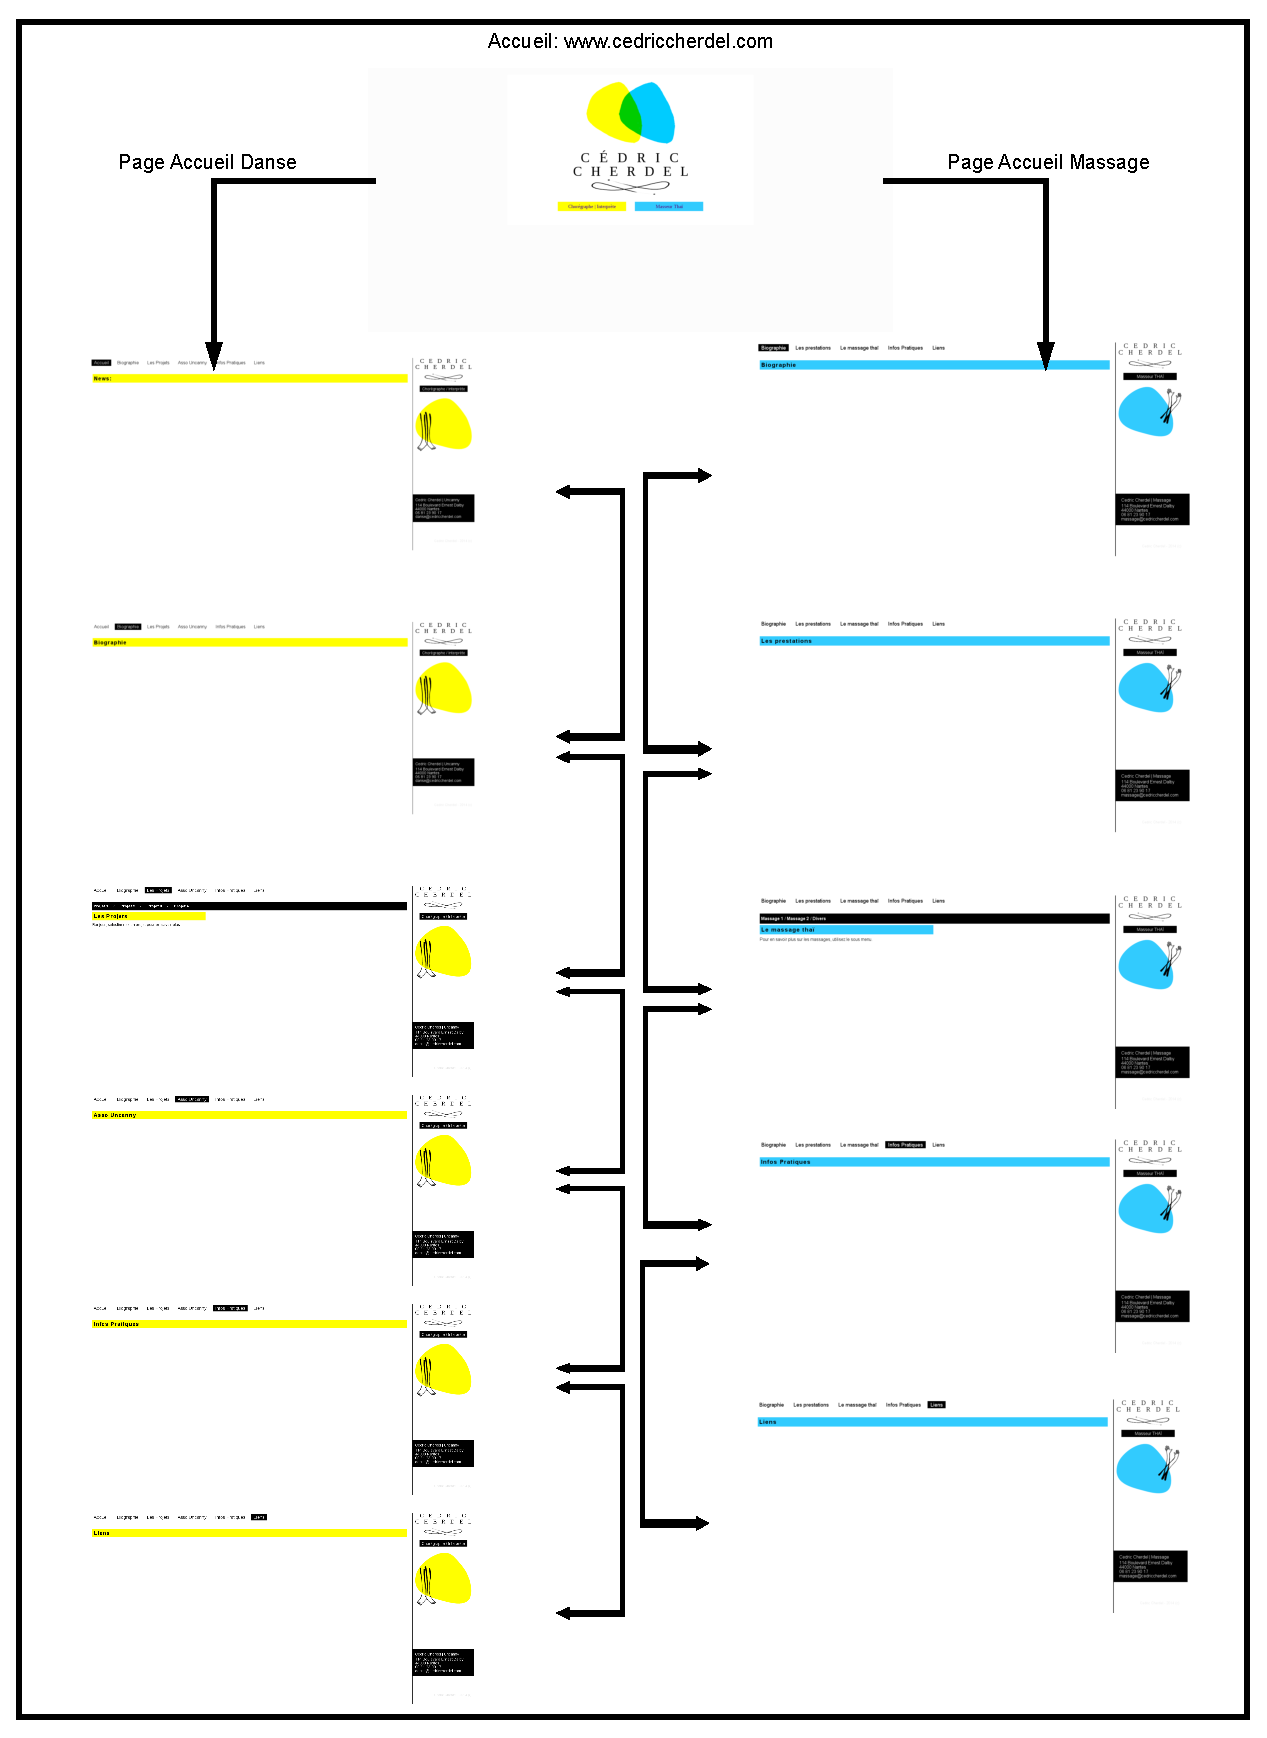
\includegraphics[width=17.5cm]{Schema-Enchainement-Pages.eps}
					\caption[Schéma d'enchainement des Pages Web]{Schéma d'enchainement des pages Web pour les sites "Accueil", "Danse" et "Massage"}
					\label{fig:Enchainement-Pages}
				\end{figure}

	\section{Test \& Qualité}
		\subsection{Fonctionnel}
			\paragraph*{}Les tests fonctionnels ont été réalisé au fil de l'eau pendant le développement. J'ai créé des posts, des projets et d'autres documents afin de tester et valider toutes les fonctionnalités. En voici un exemple:
			
			\lstset{caption=fichier Markdown d'un post}
			\begin{lstlisting}
---
layout:				post
title:				"Nouveau projet: Catalogues Des Possibles"
date:					2014-05-01 11:10:18
categories:		Projets Production

thumbnail:		'/images/possibles/1.jpg'

video:				'/videos/possibles/1.jpg'
	mp4:				'/videos/possibles/1.mp4'
	webm:				'/videos/possibles/1.webm'
	ogv:				'/videos/possibles/1.ogg'
---
Catalogue des possibles est un projet de création de pièces de danse. Ces pièces sont pensées dans des formats de courte durée. Chaque pièce expérimente un procédé d'écriture différent.
you can [get the PDF]({{ site.url }}/pdf/possibles/1.pdf) directly.
			\end{lstlisting}

			\lstset{caption=fichier Markdown d'un projet}
			\begin{lstlisting}
---
layout:						projet
title:						"Catalogues Des Possibles, CHAMPION"
date:							2014-04-01 09:00:00
Conception:				"Conception et interprétation: Cédric Cherdel"
Interpretation:     
Scenographie:			"Laurent Cebe"
Soutient:					"Ce projet est soutenu par le 783, La FABRIQUE"

pdf:							'/pdf/possibles/1.pdf'
photo:						'/images/possibles/1.jpg'
	photo2:					'/images/possibles/2.jpg'
	photo3:					'/images/possibles/3.jpg'
	photo4:					'/images/possibles/4.jpg'
---
__Catalogue des possibles,__ est un projet de création de pièces de danse. Ces pièces sont pensées dans des formats de courte durée. Chaque pièce expérimente un procédé d'écriture différent.

*La pièce CHAMPION* est une recherche sur la transformation des gestes dansés et des codes de représentation. S'inspirant d'une méthode de composition de Tatsumi Hijikata, la transformation agit comme une dissection des parties du corps, du mouvement et crée un vocabulaire nourrit par l'imaginaire.

<script>
		$("a:contains('Les Projets')").css("background-color", "black").css("color", "white");
		$("span[class='project-name-spacer']:last").css("color", "black");
</script>
			 \end{lstlisting}			 

\chapter{Développement}
	\section{Technologies}
		\paragraph*{}Les technologies utilisés lors de ce développement sont:
			\begin{itemize}
				\item HTML5
				\item CSS3
				\item Javascript + jQuery
				\item Ruby
				\item PHP (lors du prototypages et pour le développement futur)
			\end{itemize}
		\subsection{Page d'accueil}
			\paragraph*{}Le premier développement que j'ai réalisé a été une page d'accueil\footnote{\url{http://www.cedriccherdel.com}} pour le projet, le client souhaitait une page animée, mais simple, regroupant les différents éléments graphiques et les couleurs et polices utilisés pour le thème. 
				\subparagraph{Pages HTML}Nous souhaitions utiliser les nouveautés d'animation du CSS3, j'ai donc commencé par coder une simple page HTML, en voici le code:
					\lstset{caption=Page d'accueil en HTML, language=HTML, tabsize=4, stringstyle=\color{red}, keywordstyle=\color{blue}}
					\begin{lstlisting}
<!DOCTYPE html>
<html lang="fr" dir="ltr" itemscope itemtype="http://schema.org/Article">
	<head>
		<meta charset=utf-8>
		<title>Cédric Cherdel</title>
        <meta name="description" content="Page d'accueil des sites Massage et Danse de Cédric CHERDEL">
        <meta name="keywords" content="Cédric, Cedric, cédric, cedric, CHERDEL, Cherdel, cherdel, massage, danse, contemporaine, THAÏ, Thaï, thaï, THAI, Thai, thai, UNCANNY, Uncanny, uncanny">
        <meta name="viewport" content="width=device-width, initial-scale=1.0, minimum-scale=1.0">
        
        <link rel="stylesheet" media="all" href="css/reset.css">
        <link rel="stylesheet" media="all" href="css/styles.css">

        <link rel="shortcut icon" href="imgs/identity/favicon.ico">
        <link rel="apple-touch-icon" href="imgs/identity/CC_Badge_64.png">
        <link rel="apple-touch-icon-precomposed" href="imgs/identity/CC_Badge_64.png">

        <script src="js/jquery-2.1.1.min.js"></script>

        <!--[if lt IE 9]>
            <script src="http://html5shim.googlecode.com/svn/trunk/html5-els.js"></script>
        <![endif]-->

    </head>
    <body>
		<div id="main">
	        <header>
				<figure id="logo">
					<a href="http://danse.cedriccherdel.com" id="jaune" title="Chorégraphe | Interprète"></a>
					<a href="http://massage.cedriccherdel.com" id="bleu" title="Masseur THAÏ"></a>
				</figure>
				<hgroup>
					<h1 id="prenom">cédric</h1>
					<h1 id="nom">cherdel</h1>
				</hgroup>
				<div id="boucle"></div>
    	    </header>
        	<nav>
		        <ul>
    		        <li><a href="http://danse.cedriccherdel.com" id="danse_menu">chorégraphe | interprète</a></li>
        	        <li><a href="http://massage.cedriccherdel.com" id="massage_menu">masseur thaï</a></li>
        	    </ul>
        	</nav>
			<footer>
				<p>Copyright <address><a href="mailto:webmaster@cedriccherdel.com">Cédric CERDEL</a></address> 2014</p>
			</footer>
		</div>
		<script src="js/accueil.js"></script>
    </body>
</html>					
					\end{lstlisting}
					Je fais appel dans la partie <head> de cette page à deux fichiers CSS et deux fichiers Javascript, dans le <body> je charge mon propre fichier Javascript qui servira à l'animation. La syntaxe est très simple, j'utilise une première <div> qui a comme id "main" qui me servira à centrer la page dans la fenêtre du navigateur. Puis j'utilise les nouvelles balises HTML5 <header>, <figure>, <hgroup>, <nav> et <footer>. Ces nouvelles balises sont là pour mieux structurer le document, ce qui permet une meilleur compréhension du code de la page par les moteurs de recherches. Tout est fait ici pour favoriser un référencement naturel de ce site.

				\subparagraph{Javascript \& jQuery}Le premier fichier JS sert à ajouter la bibliothèque jQuery (ligne 17), le second, fournis par Google, sert à ajouter aux anciens navigateurs les nouvelles balises HTML5, ce qui permet de maximiser la compatibilité (lignes 19 à 21).\\
				Le dernier fichier Javascript, simple mais efficace, sert à animer la page, en voici le code source:
					\lstset{caption=fichier accueil.js, language=java, tabsize=4, stringstyle=\color{blue},}
					\begin{lstlisting}
jQuery('#jaune').mouseenter(function() {jQuery('#logo').css('background','url("imgs/Jaune-Danse.png") no-repeat 0 0'),
	jQuery('#danse_menu').css('color','black').css('background-color','white').css('border','solid 1px #FFFF00')});
jQuery('#jaune').mouseleave(function() {jQuery('#logo').css('background','url("imgs/Deux-Couleurs.png") no-repeat 0 0'),
	jQuery('#danse_menu').css('color','#000').css('background-color','#FFFF000').css('border','solid 1px white')});

jQuery('#bleu').mouseenter(function() {jQuery('#logo').css('background','url("imgs/Bleu-Massage.png") no-repeat 0 0'),
	jQuery('#massage_menu').css('color','black').css('background-color','white').css('border','solid 1px #32CBFE')});
jQuery('#bleu').mouseleave(function() {jQuery('#logo').css('background','url("imgs/Deux-Couleurs.png") no-repeat 0 0'),
	jQuery('#massage_menu').css('color','#000').css('background-color','#32CBFE').css('border','solid 1px white')});


jQuery('#danse_menu').mouseenter(function() {jQuery('#logo').css('background','url("imgs/Jaune-Danse.png") no-repeat 0 0'),
	jQuery('#danse_menu').css('color','black').css('background-color','white').css('border','solid 1px #FFFF00')});
jQuery('#danse_menu').mouseleave(function() {jQuery('#logo').css('background','url("imgs/Deux-Couleurs.png") no-repeat 0 0'),
	jQuery('#danse_menu').css('color','#000').css('background-color','#FFFF00').css('border','solid 1px white')});

jQuery('#massage_menu').mouseenter(function() {jQuery('#logo').css('background','url("imgs/Bleu-Massage.png") no-repeat 0 0'),
	jQuery('#massage_menu').css('color','black').css('background-color','white').css('border','solid 1px #32CBFE')});
jQuery('#massage_menu').mouseleave(function() {jQuery('#logo').css('background','url("imgs/Deux-Couleurs.png") no-repeat 0 0'),
	jQuery('#massage_menu').css('color','#OOO').css('background-color','#32CBFE').css('border','solid 1px white')});

jQuery('#prenom').animate({opacity: 1, top: "-=25px"},{duration: 800});
jQuery('#nom').animate({opacity: 1, top: "+=25px"},{duration: 800});
jQuery('figure').delay(1300).animate({opacity: 1},{duration: 800});
jQuery('nav').delay(1300).animate({opacity: 1},{duration: 800});
jQuery('#boucle').delay(1000).animate({opacity: 1},{duration: 800});
					\end{lstlisting}	
				\subparagraph*{}Dans les lignes 1 à 20, j'utilise plusieurs sélecteurs CSS avec jQuery qui me permettent d'animer les rollovers des boutons en même temps qu'un rollover sur le logo, ce qui permet au choix, de survoler les boutons et d'avoir en plus de son animation, l'animation du logo, ou de survoler le logo et d'avoir l'animation du bouton correspondant.\\
				Pour cela, après avoir sélectionné mon élément (jQuery('\#jaune')), j'utilise la fonction jQuery ".mouseenter(...)" qui permet d'activer le code contenu entre parenthèses lors du survol. Dans ces parenthèses, je déclare une fonction anonyme, qui, via d'autres sélecteurs, ajoute (ou modifie dans notre cas) des propriétés CSS (exemple: 'background','url("imgs/Jaune-Danse.png").\\
				Je répète l'opération pour les trois autres éléments à animer.
				\subparagraph*{}Les lignes 22 à 26 servent à animer les différents éléments. On trouve dans l'ordre, le prénom qui apparait et se décale de 25px vers le haut, le nom qui apparait et se décale de 25px vers le bas, les logos et menu qui apparaissent en dernier grâce à la fonction ".delay(1300)" qui prend en paramètre une durée en milliseconde (soit 1,3 seconde), et la "boucle" qui souligne le texte déjà présent et apparait au bout d'une seconde.
				\subparagraph*{}Toutes ces fonctions (sélecteurs, délais, animate, css et mouseenter) sont fournis par la bibliothèque jQuery, on trouve toutes la documentations avec des exemples d'utilisation sur le site officiel\footnote{\url{http://api.jquery.com/}}.

				\subparagraph{CSS}Le premier fichier CSS (reset.css) sert à remettre à zéro tout les éléments html, il a été créé par Eric Meyer\footnote{\url{http://cssreset.com}}. Le second fichier (styles.css) de cette page sera utilisé pour débuter le thème. voici son code source:
					\lstset{caption=fichier styles.css, language=HTML, tabsize=4, stringstyle=\color{blue}}
					\begin{lstlisting}
/* Windows Minimum width: 900px */

body {
	overflow-x: hidden;
	overflow-y: scroll;
	font-size: 12px;
	font-family: Times New Roman, serif;
	background-color: #FCFCFC;
}

#main {
	width: 900px;
	height: 550px;
	margin: 0px auto;
	background-color: white;
}

header {
	text-align: center;
	margin-top: 25px;
	padding-top: 25px;
}
figure {
	opacity: 0;
}

#logo {
	width: 325px;
	height: 228px;
	margin: 0px auto;
	background: url("../imgs/Deux-Couleurs.png") no-repeat 0 0;
	position: relative;
}

#jaune, #bleu {
	display: inline-block;
	position: relative;
}

#jaune {
	width: 120px;
	height: 228px;
	top: 0px;
	left: -40px;
}

#bleu {
	width: 120px;
	height: 228px;
	top: 0px;
	left: 40px;
}

hgroup {
	height: 100px;
}

h1 {
	text-transform: uppercase;
	font-size: 4.2em;
}
#prenom {
	margin-top: 25px;
	margin-left: 29px;
	letter-spacing: 35px;
	opacity: 0;
	position: relative;
	top: 25px;
}
#nom {
	margin-top: 0px;
	margin-left: 34px;
	letter-spacing: 32px;
	opacity: 0;
	position: relative;
	top: -25px;
}

#boucle {
	width: 286px;
	height: 56px;
	margin: 5px auto;
	background-image: url("../imgs/Boucle-Accueil.png");
	opacity: 0;
}

nav {
	text-align: center;
	text-transform: capitalize;
	font-size: 1.5em;
	margin-top: 25px;
	opacity: 0;
}

ul {
	margin-left: -25px;
}

li {
	display: inline-block;
}

li a {
	display: block;
	color: #OOO;
	text-decoration: none;
	width: 250px;
	padding: 8px 0px;
	margin-left: 25px;
	border: solid 1px white;
	background-color: grey;	
}

#danse_menu {
    background-color: #FFFF00;
}

#massage_menu {
    background-color: #32CBFE;
}

li a:hover {
	color: black;
	background-color: white;
	border: solid 1px black;
}

footer {
	display: none;
}
					\end{lstlisting}
				\subparagraph*{}Je commence par modifier l'apparence du corps de la page (body), puis je donne la taille souhaité à ma première balise <div> et j'en profite pour center ce conteneur dans la page. J'utilise ensuite les nouvelles balises HTML5 pour centrer le texte dans le bloc, et pour définir l'opacité du texte à 0 (sur l'image 1 de la timeline). J'ajoute mon logo et je le centre, puis je modifie la taille et la position des deux zones cliquables du logo. Je travaille ensuite le texte et les autres éléments.\\
				Enfin, je défini la propriété "display" sur "none" pour caché le <footer>, car il n'est utilisé que pour le référencement. En effet, d'après plusieurs pages Google (sur l'aide au développement et sur html5rocks\footnote{\url{http://www.html5rocks.com/en/}}), il est indiqué qu'une page ayant un <footer> principal avec une balise <address> est mieux référencé par le moteur.
				\newpage

		\subsection{Thème}
			\paragraph{CSS}Les thèmes des deux sites étant très proche, je me suis focalisé sur le développement du thème du site danse\footnote{\url{http://danse.cedriccherdel.com}}. J'ai donc produits un fichier CSS très proche du précédent.

		\subsection{Site danse}
			\paragraph{JekyllRB}
				\subparagraph{Introduction}JekyllRB est un CMS un particulier pour plusieurs raisons:
					\begin{itemize}
						\item Il est basé sur Ruby (plus précisément Ruby on Rails)
						\item Il génère un site statique et n'as donc pas besoin de moteur de base de données
						\item Il a été pensé dans une otique de simplicité (on ne passe pas des heures à mettre en forme, on se focalise sur le contenu)
						\item Il s'installe en quelques secondes
						\item La plus part des actions que l'on retrouve dans un CMS comme Wordpress sont automatisé
						\item Il utilise pour la rédaction de nouveau post le Markdown ou le HTML
						\item Il a été pensé comme moteur de blog, il gère donc par défaut les tags, les catégories, des pages statiques, des posts et les permaliens.
					\end{itemize}
				\subparagraph{Installation}Il est nécessaire d'avoir Ruby 2 installé sur sa machine. Il est ensuite très simple à mettre en place avec trois simples lignes :
					\lstset{language=bash, tabsize=4}
					\begin{lstlisting}
~ $ gem install jekyll
~ $ jekyll new myblog & cd myblog
~/myblog $ jekyll serve
					\end{lstlisting}
					La première ligne installe Jekyll, la seconde, créer un nouveau site (on retrouve ce genre de syntaxes avec les framework Zend et Symfony) et la troisième ligne permet de lancer le serveur web intégré à Jekyll.\\
					Ce serveur ne remplace absolument pas un serveur web de production comme NGINX ou Apache, mais permet de tester son développement en local.\\
					Le site est maintenant visible à cette adresse : \url{http://localhost:4000}.
				\subparagraph{Architecture}L'architecture de Jekyll est assez simple, par défaut, lors de la création d'un nouveau site, plusieurs fichiers et dossiers sont généré.
					\lstset{caption=arborescences du site généré par JekyllRB , numbers=none, language=bash, tabsize=4, frame=none, backgroundcolor=\color{white}}
					\begin{lstlisting}
								.
								|-- about.md
								|-- _config.yml
								|-- css
								|    '-- main.css
								|-- feed.xml
								|-- _includes
								|    |-- footer.html
								|    |-- header.html
								|    '-- head.html
								|-- index.html
								|-- _layouts
								|    |-- default.html
								|    |-- page.html
								|    '-- post.html
								|-- _posts
					     			 '-- 2014-06-01-welcome-to-jekyll.markdown
					\end{lstlisting}
				\subparagraph*{}
					\begin{itemize}
						\item Le fichier "about.md" est un exemple de page statique
						\item Le fichier "\_config.yml" contient tout les paramètres globaux du site.
						\item On trouve aussi un dossier "css" contenant un fichier "main.css" utilisé par le thème par défaut, on peut le remplacer ou le modifier en fonction de nos besoins.
						\item Le fichier "feed.xml" est en générateur de flux RSS que l'on peut réutilisé (dans notre cas, on va simplement le supprimer).
						\item Les dossier préfixé d'un "\_" ne seront pas déployé dans le site mais contiennent les éléments servant à la génération des du site.
						\item Le dossier "\_include" contient trois fichiers HTML qui composeront les pages généré.
						\item Le fichier "index.html" est la page d'accueil du site contenant les liens vers les posts de ce blog.
						\item Le dossier "\_layout" contient les mises en pages utilisables.
						\item Enfin, le dossier "\_posts" contient les articles du site.
					\end{itemize}

			\paragraph{Explications}
				\subparagraph{Fichier index.html}Voici son code source:
					\lstset{caption=Fichier "index.html" généré par JekyllRB , language=ruby, tabsize=4, numbers=left, stepnumber=1, frame=single, breaklines=true, backgroundcolor=\color{lightgray},}
					\begin{lstlisting}
---
layout: default
---

<div class="home">

	<h1>Posts</h1>

	<ul class="posts">
		
		<li>
			<span class="post-date">{{ post.date | date: "%b %-d, %Y" }}</span>
			<a class="post-link" href="{{ post.url | prepend: site.baseurl }}">{{ post.title }}</a>
		</li>
		
	</ul>

	<p class="rss-subscribe">subscribe <a href="{{ "/feed.xml" | prepend: site.baseurl }}">via RSS</a></p>

</div>
					\end{lstlisting}
				\subparagraph*{}La première partie (lignes 1 à 3), permet de sélectionner le layout utilisé pour cette page.\\
				Les lignes 5, 7 et 9 sont les balises HTML qui seront utilisé dans la génération de la page.\\
				La ligne 10 est du ruby, cette boucle permet de générer la liste des posts disponibles dans le dossier "posts" grâce à l'utilisation du mot clef "site.posts". Comme on le voit ici, il est très simple d'ajouter du contenu rapidement, si on souhaite créer une autre liste d'article, on créer un dossier préfixé d'un "\_" par exemple "\_newPosts" et on utilise le mot clef "site.newPosts".
				\subparagraph*{}L'utilisation de doubles accolades (\{\{ \}\}) dans les lignes 12, 13 et 18 permet de remplacer ces portions de code lors de la génération des pages. Dans le cas de la ligne 12, le code \{\{ post.date | date "\%b \%-d, \%Y" \}\} produira, lors de la génération, la date du post renseigné dans ce dernier formaté en: "mois jour, Année" soit par exemple "05 28, 2014". L'utilisation du "tube" (|) permet de modifier la génération précédente comme on le fait dans un shell.
				\subparagraph*{}Le mot clef "post.url" est à noter, il permet de générer l'adresse web du post qui sera intégré dans cette liste.\\
				Enfin, le mot clef "site.baseurl" est aussi très important, il permet de préfixer le une adresse web par l'adresse du site ce qui donne au final une adresse web correctement formaté.

				\subparagraph{Fichier post.html}Voici son code source:
					\lstset{caption=Fichier "post.html" généré par JekyllRB, language=HTML}
					\begin{lstlisting}
---
layout: default
---
<div class="post">

	<header class="post-header">
		<h1>{{ page.title }}</h1>
		<p class="meta">{{ page.date | date: "%b %-d, %Y" }} - {{ page.author }} - {{ page.meta }}</p>
	</header>

	<article class="post-content">
		{{ content }}
	</article>
					\end{lstlisting}
				\subparagraph*{}On peut voir à la ligne 8 l'introduction d'une condition (\{\% if page.author \%\}) qui permet d'ajouter le nom de l'auteur du post si celui-ci est renseigné dans ce dernier. Pour créer un tel mot clef, il suffit dans le fichier du post, dans la première partie (entre les --- ---) d'ajouter un mot clef, par exemple "superMotClef" suivit de ":" et de mettre le texte (ou code) que l'on souhaite intégrer. Il est donc très simple, par exemple pour un post d'ajouter un fichier joint uniquement lors ce que celui-ci est présent.

		\subsection{Code du site}
			\paragraph{Fichiers}J'ai créer six fichiers:
				\begin{enumerate}
					\item \textbf{"1\_index.html"}:			Page d'accueil du site contenant les dernières news du site.
					\item \textbf{"2\_biographie.md"}: 		Page statique contenant une biographie.
					\item \textbf{"3\_projets.html"}:		Page d'accueil des projets passés, en cours et futurs.
					\item \textbf{"4\_uncanny.md"}:			Page statique présentant l'association.
					\item \textbf{"5\_infos-pratiques.md"}:	Page statique avec les infos pratiques.
					\item \textbf{"6\_liens.md"}:			Page statique contenant des liens relatifs au projet ou à la compagnie de danse.
				\end{enumerate}
			Ces fichiers sont préfixé d'un numéro ce qui permet de générer le menu du site dans l'ordre des fichiers. Encore une fois, on voit que Jekyll nous facilite le travail.
			\paragraph{dossiers}J'ai aussi créer plusieurs dossiers:
				\begin{enumerate}
					\item \textbf{\_draft}:					Dossier un peu particulier, l'intégralité des fichiers contenus ne seront pas publiés.
					\item \textbf{images}:					On mettra ici toutes les images que l'on souhaite intégrer dans les posts ou projets (Ce dossier n'étant pas préfixé, il sera ajouté au site généré).
					\item \textbf{js}:						Dossier contenant les fichiers Javascripts utiles au site.
					\item \textbf{\_locales}:				Dossier contenant un fichier de traduction (fr.yml) des mots générés par Jekyll. Cette traduction sera principalement utilisé pour formater les dates en français.
					\item \textbf{pdf}:						Ici se trouverons les fichiers pdf joints au projets.
					\item \textbf{\_plugins}:				Dans ce dossier, nous ajouterons les greffons nécessaires (notamment un parser permettant d'utiliser le fichier de traduction.)
					\item \textbf{\_projets}:				Dossier créer pour ajouter les projets (ce dossier doit être déclaré dans le fichier "\_config.yml").
					\item \textbf{sources}:					Ici nous avons les images utilisés dans le CSS du site, nous y ajouterons les autres éléments graphiques lors ce que ceci seront finis.
					\item \textbf{video}:					Enfin, on ajoutera ici les vidéos intégrés dans les projets.
				\end{enumerate}
			\paragraph{Base de données}Comme tout blog, on utilise ici une base de données, celle-ci est très simple, elle utilise une arborescence de dossier, qui dans une SGBD traditionnel correspondrais aux tables, et des fichiers plats (Markdown (extension ".markdown" ou ".md") ou HTML), qui correspondent aux entrées dans les tables.\\
			Ce système permet une sauvegarde rapide, une modification des entrées tout aussi rapide, mais implique une rigueur dans la gestion des fichiers. En effet, l'absence de moteur implique que la perte d'un article est possible, il suffit d'une simple suppression !\\
			L'autre avantage est qu'il est très aisé de migrer vers un autre CMS, l'utilisation de scripts bash, disponible sur internet ou facilement développable, permet une intégration facile dans MySQL ou PostgreSQL des posts et autres éléments.
			\paragraph{Fichier layout default.html}Ce fichier est utilisé pour toutes les pages car c'est le squelette de base du site:
				\lstset{caption=Fichier "default.html", language=HTML}
				\begin{lstlisting}
<!DOCTYPE html>
<html>

  

    <body>

    
        

    <div class="page-content">
      {{ content }}
    </div>

    

    </body>
</html>

				\end{lstlisting}
			\paragraph{Fichier layout projet.html}Ce fichier est intéressent dans son développement, on y utilise plusieurs conditions en fonctions des éléments renseignés dans le fichier de projet. Voici le code que j'ai réalisé pour cette nouvelle catégorie de "post":
				\lstset{caption=Fichier "projet.html"}
				\begin{lstlisting}
---
layout: default
---
<div class="home">

	<ul class="submenu">
 		
		<li>
			<a class="project-name" href="{{ post.url | prepend: site.baseurl }}">{{ post.title }}</a><span class="project-name-spacer">/<span>
		</li>
		
	</ul>
	
	<section class="subsection-content">
	
		<article class="left">
			<header>{{ page.title }}</header>
			{{ content }}
			
			<footer>
				<a href="{{ site.url }}{{ page.pdf }}" class="dossier">Télécharger le dossier</a>
			</footer>
			
		</article>
		
		<aside class="right">
			
			<figure class="picture">
				<img src="{{ site.url }}{{ page.photo }}" alt="{{ page.title }}">
			</figure>
			
			 <section class="project-infos">{{ page.Conception }}</section>
			 <section class="project-infos">{{ page.Interpretation }}</section>
			 <section class="project-infos">{{ page.Scenographie }}</section>
			 <section class="project-infos">{{ page.Soutient }}</section>
			
			
			<figure id="video" class="player-video">
				<video width="806px" height="398px" preload="auto" controls poster="{{ site.url }}{{page.videoThumb}}">
				<source src="{{ site.url }}{{page.mp4}}" type='video/mp4; codecs="avc1.42E01E, mp4a.40.2"' />
				<source src="{{ site.url }}{{page.webm}}" type='video/webm; codecs="vp8, vorbis"' />
				<source src="{{ site.url }}{{page.ogv}}" type='video/ogg; codecs="theora, vorbis"' />
				</video>
			</figure>
			
		</aside>
	
	</section>
	
</div>

				\end{lstlisting}
				\subparagraph{}On remarque en ligne 7 que j'utilise le mot clef "site.projets" se référent au dossier "\_projets". Dans les lignes 6 à 12, on créé un sous menu avec les noms des projets disponibles.
				\subparagraph{}Entre les lignes 16 et 24, on génère le texte descriptif du projet, avec un <header> comprenant le titre du projet, le contenu (\{\{ content \}\}), et un <footer> pour cette article contenant le lien de téléchargement du dossier pdf du projet.\\
				Cette balise est entouré d'une condition, qui test si un fichier pdf est présent dans la description du projet, ce qui permet d'ajouter automatiquement le fichier si il est présent.
				\subparagraph{}Dans les lignes 27 à 31, on utilise la même technique pour ajouter automatiquement des photos, si une photo est présente, elle est ajouté et si plusieurs sont disponibles, un greffon créé automatiquement un carrousel.
				\subparagraph{}À l'heure actuel, le développement de ce greffon est toujours en cours, il se base sur JekyllGalleryTag\footnote{\url{https://github.com/redwallhp/JekyllGalleryTag}} et FancyBox\footnote{\url{http://fancyapps.com/fancybox/}}
				\subparagraph{}Les lignes 32, 33, 34 et 35 permettent d'ajouter des information sur le projets si elles sont disponibles.
				\subparagraph{}Enfin, entre les lignes 37 à 45, on ajoute, toujours si ces fichiers sont disponibles, la vidéo du projet. Cette vidéo peut être disponible en trois format de fichiers, le premier pour les produits Apple et Microsoft, le deuxième format pour les navigateurs Google et le dernier format pour les navigateurs Mozilla. On ajoute aussi un thumbnail pour le lecteur.
				\subparagraph{}On voit dans ce fichier que l'ajout "automatique" de fichiers dans une page peut être très rapidement réalisé, c'est pour moi une des forces de JekyllRB, qui reste dans la philosophie de développement UNIX du KISS\footnote{\url{https://fr.wikipedia.org/wiki/Principe_KISS}}.
			\paragraph{Fichier header.html}Ce fichier (que l'on trouve dans le dossier "\_include") contient le début du <body> HTML, on retrouve le menu de navigation.
			\paragraph{Fichier side.html}Ce fichier (que l'on trouve dans le dossier "\_include") contient toute la sidebar du site, on retrouve le titre du site, diverses informations et un peu de graphisme. Il a été pensé dans l'esprit d'un marque page. Cette sidebar est présente sur toutes les pages du site.
			\paragraph{Fichier main.css}Ce fichier est basé sur le fichier créé pour la page d'accueil
				\lstset{caption=Fichier "main.css", language=HTML}
				\begin{lstlisting}
html, body, div, span, object, iframe, h1, h2, h3, h4, h5, h6, p, blockquote, pre, abbr, address, cite, code, del, dfn, em, img, ins, kbd, q, samp, small, strong, sub, sup, var, b, i, dl, dt, dd, ol, ul, li, fieldset, form, label, legend, table, caption, tbody, tfoot, thead, tr, th, td, article, aside, canvas, details, figcaption, figure, footer, header, hgroup, menu, nav, section, summary, time, mark, audio, video {
    /*background: none repeat scroll 0 0 rgba(0, 0, 0, 0);*/
	background: white;
    border: 0 none;
    font-size: 100%;
    margin: 0;
    outline: 0 none;
    padding: 0;
    vertical-align: baseline;
}
body {
    line-height: 1;
}
article, aside, details, figcaption, figure, footer, header, hgroup, menu, nav, section {
    display: block;
}
nav ul {
    list-style: none outside none;
}
blockquote, q {
    quotes: none;
}
blockquote:before, blockquote:after, q:before, q:after {
    content: none;
}
a {
    background: none repeat scroll 0 0 rgba(0, 0, 0, 0);
    font-size: 100%;
    margin: 0;
    padding: 0;
    text-decoration: none;
    vertical-align: baseline;
}
hr {
    -moz-border-bottom-colors: none;
    -moz-border-left-colors: none;
    -moz-border-right-colors: none;
    -moz-border-top-colors: none;
    border-color: #CCCCCC -moz-use-text-color -moz-use-text-color;
    border-image: none;
    border-right: 0 none;
    border-style: solid none none;
    border-width: 1px 0 0;
    display: block;
    height: 1px;
    margin: 1em 0;
    padding: 0;
}
input, select {
    vertical-align: middle;
}
html {
}
html, body { 
    height: 100%; 
    font-family: arial;
    margin: 10px auto;
    max-height: 900px;
    width: 1600px;
}
.site-nav .menu-icon {
    display: none;
}
.site-header {
    /*background-color: #FFFFFF;*/
    height: 20px;
    padding: 10px 5px 5px;
    width: 1270px;
}
.page-link {
    color: #000000;
    font-size: 1.2em;
    margin-right: 20px;
    margin-left: -10px;
    padding: 2px 10px;
}
.page-link:hover {
    background-color: #000000;
    color: #FFFFFF;
}

.home ul {
	list-style-type: none;
}

.post-date {
	margin-top: 5px;
	display: inline-block;
}
.post-content, .post {
	padding-top: 10px;
    color: black;
}
.post-content p {
	padding-bottom: 15px;
	line-height: 1.2em;
}

.left {
    /*background-color: #FF6347;*/
	margin-top: 5px;
	display: block;
    height: 400px;
    overflow-y: auto;
    width: 460px;
}
.left header, .home h1, .post-header h1 {
    background-color: #FFFF00;
    font-weight: bold;
    letter-spacing: 2px;
    padding: 5px;
	font-size: 1.3em;
	margin-bottom: 10px;
	line-height: 1.2em;
    color: #000;
}
.home h1 {
	margin-top: 10px;
}
.left p {
    padding: 0 10px 15px 0;
    text-align: justify;
}

.right {
    /*background-color: #D8BFD8;*/
    display: block;
    height: 400px;
    margin-left: 470px;
    margin-top: -400px;
    width: 810px;
}

.picture {
	text-align: right;
}

.submenu {
    background-color: #000000;
    color: #FFFFFF;
    padding: 10px 5px;
	margin-top: 11px;
}
.submenu li {
    display: inline-block;
}

.project-name {
    color: #FFFFFF;
    font-size: 1em;
    font-weight: bold;
	background-color: black;
}
.project-name-spacer {
	color: #FFF;
	background-color: #000;
	display: inline-block;
	padding: 0 20px;
}
.page-content {
    margin-top: -725px;
    width: 1280px;
}
.dossier {
    background-color: #000000;
    color: #FFFFFF;
    padding: 5px;
}
.project-infos:first-of-type {
	margin-top: 10px;
}
.project-infos {
	font-size: 0.9em;
    text-align: right;
}

#sidebar {
    /*background-color: #FF6347;*/
    border-left: 2px solid black;
	border-right: 2px solid white;
    display: block;
    height: 780px;
    margin-left: 1300px;
    margin-top: -35px;
    padding-left: 10px;
    text-align: center;
    width: 230px;
}
#side-title {
    font-family: times new roman;
    font-size: 1.5em;
    font-weight: normal;
	margin-bottom: 10px;
	text-align: right;
	margin-right: 3px;
}
#prenom, #nom {
    display: block;
    letter-spacing: 20px;
}
#boucle {
    /*background-color: #EE82EE;
    margin-left: -20px;*/
	padding-top: 5px;
	padding-bottom: 5px;
}
#boucle > img {
    width: 155px;
}
#side-subtitle {
    background-color: #000000;
    color: #FFFFFF;
    margin: 10px auto 15px;
    padding: 5px 0;
    width: 195px;
}
#side-main-menu > a {
    color: #000000;
    margin-left: -120px;
    text-decoration: none;
}
#side-main-menu > a:hover {
    background-color: #000000;
    color: #FFFFFF;
    padding: 5px;
    text-decoration: underline;
}
#side-main-menu > figure {
    height: 380px;
}
#side-address {
    background-color: #000000;
    color: #FFFFFF;
    margin: 20px -10px 0;
    padding: 15px 10px;
    text-align: left;
    width: 230px;
}
p#side-address a {
    color: white;
}
.side-address-subtitle {
    background-color: #000000;
    color: #FFFFFF;
    display: inline-block;
    margin: 0 0 5px;
    padding: 0;
}

.site-footer {
    /*background-color: #EE82EE;
    bottom: -593px;
    display: block;
    font-size: 0.75em;
    padding: 10px 0;
    position: relative;
    text-align: center;
    top: auto;
    width: 1280px;*/
}
.site-footer a {
    color: #000000;
}

.copyright {
	text-align: right;
	margin-top: 70px;
	font-size: 0.8em;
	color: #E8E8E8;
}

/* ----------------------------------------------------------*/
/* --------------------- media queries --------------------- */
/* ----------------------------------------------------------*/

@media screen and (max-width: 750px) {

  .footer-col-1 { width: 50%; }

  .footer-col-2 {
    width: 45%; /*fallback*/
    width: -webkit-calc(50% - 10px);
    width: -moz-calc(50% - 10px);
    width: -o-calc(50% - 10px);
    width: calc(50% - 10px);
    margin-right: 0;
  }

  .site-footer .column.footer-col-3 {
    width: auto;
    float: none;
    clear: both;
  }

}

@media screen and (max-width: 600px) {

  .wrap { padding: 0 12px; }

  .site-nav {
    position: fixed;
    z-index: 10;
    top: 14px; right: 8px;
    background-color: white;
    -webkit-border-radius: 5px;
    -moz-border-radius: 5px;
    border-radius: 5px;
    border: 1px solid #e8e8e8;
  }

  .site-nav .menu-icon {
    display: block;
    font-size: 24px;
    color: #505050;
    float: right;
    width: 36px;
    text-align: center;
    line-height: 36px;
  }

  .site-nav .menu-icon svg { width: 18px; height: 16px; }

  .site-nav .trigger {
    clear: both;
    margin-bottom: 5px;
    display: none;
  }

  .site-nav:hover .trigger { display: block; }

  .site-nav .page-link {
    display: block;
    text-align: right;
    line-height: 1.25;
    padding: 5px 10px;
    margin: 0;
  }

  .post-header h1 { font-size: 36px; }
  .post-content h2 { font-size: 28px; }
  .post-content h3 { font-size: 22px; }
  .post-content h4 { font-size: 18px; }
  .post-content blockquote { padding-left: 10px; }
  .post-content ul,
  .post-content ol { padding-left: 10px; }

 .site-footer .column {
    float: none;
    clear: both;
    width: auto;
    margin: 0 0 15px; }

}
				\end{lstlisting}

\chapter{Déploiement}
	\section{Prérequis techniques}
		\paragraph{}Sur le serveur : Un serveur web (ex: Apache, NGINX)et un accès FTP.\\
		Sur la machine de génération du site : Ruby 2, un éditeur de texte et un client FTP.
	%\section{Scripts de mise en place de l'architecture logiciels}
	%\section{Scripts de déploiement de l'application}
	\section{Documentation:}
		\subsection{Développeur}L'utilisation des documentations officiels de JekyllRB\footnote{\url{http://jekyllrb.com/docs/home/}}, de jQuery\footnote{\url{http://api.jquery.com}} ainsi que de Ruby on Rails\footnote{\url{http://rubyonrails.org/}} sont recommandé, on y trouve tout le éléments présent dans ce développement complété par beaucoup d'exemple.
		\subsection{Administrateur}Une documentation sur l'administration générale et l'ajout de projet sera disponible en vidéo (screencast) depuis le wiki du projet.

\chapter{Bilan \& Conclusion}
	\paragraph*{}Ce stage m'as permis d'acquérir de nouvelles compétences aussi bien au niveau théorique que pratique. J'ai pu améliorer mes connaissances sur Ruby et sur HTML5. Enfin, j'ai découvert le monde de la Danse contemporaine ainsi que les éléments nécessaires à la mise en place d'un spectacle.
	\paragraph*{}En effet, cette période de deux mois au sein de cette association m'a permis:
	\begin{itemize}
		\item De mieux connaitre le milieu associatif
		\item D'étendre mes connaissances acquises lors de la formation en réalisant un thème JekyllRB en tenant compte des contraintes de mis en pages sur différentes plateformes
		\item D'utiliser les nouveautés d'animation en HTML5 pour la pages d'accueil
		\item D'utiliser la librairie jQuery
		\item D'avoir une meilleur vision des contraintes lié à un développement spécifique
	\end{itemize}
	\paragraph*{}La réalisation de ces tâches, l'aide de la communauté de Stack Overflow et l'implication des différents acteurs de ce stage, m'a permis d'atteindre les objectifs demandés, de devenir plus autonome et opérationnel dans le développement web, d'exploiter mes connaissances et d'en acquérir de nouvelles.
	\paragraph*{}Pour finir, je suis convaincu que cette expérience me permettra d'être plus en adéquation avec le marché de l'emploi dans la région.

\chapter{Liste des Annexes}
	\begin{enumerate}
		\item CV
		\item Contenu pédagogique
		\item Présentation du titre
		\item RC
		\item REAC
		\item Cahier des Charges
	\end{enumerate}

%\listoffigures

\end{document}
